% Options for packages loaded elsewhere
% Options for packages loaded elsewhere
\PassOptionsToPackage{unicode}{hyperref}
\PassOptionsToPackage{hyphens}{url}
\PassOptionsToPackage{dvipsnames,svgnames,x11names}{xcolor}
%
\documentclass[
  letterpaper,
  DIV=11,
  numbers=noendperiod]{scrreprt}
\usepackage{xcolor}
\usepackage{amsmath,amssymb}
\setcounter{secnumdepth}{5}
\usepackage{iftex}
\ifPDFTeX
  \usepackage[T1]{fontenc}
  \usepackage[utf8]{inputenc}
  \usepackage{textcomp} % provide euro and other symbols
\else % if luatex or xetex
  \usepackage{unicode-math} % this also loads fontspec
  \defaultfontfeatures{Scale=MatchLowercase}
  \defaultfontfeatures[\rmfamily]{Ligatures=TeX,Scale=1}
\fi
\usepackage{lmodern}
\ifPDFTeX\else
  % xetex/luatex font selection
\fi
% Use upquote if available, for straight quotes in verbatim environments
\IfFileExists{upquote.sty}{\usepackage{upquote}}{}
\IfFileExists{microtype.sty}{% use microtype if available
  \usepackage[]{microtype}
  \UseMicrotypeSet[protrusion]{basicmath} % disable protrusion for tt fonts
}{}
\makeatletter
\@ifundefined{KOMAClassName}{% if non-KOMA class
  \IfFileExists{parskip.sty}{%
    \usepackage{parskip}
  }{% else
    \setlength{\parindent}{0pt}
    \setlength{\parskip}{6pt plus 2pt minus 1pt}}
}{% if KOMA class
  \KOMAoptions{parskip=half}}
\makeatother
% Make \paragraph and \subparagraph free-standing
\makeatletter
\ifx\paragraph\undefined\else
  \let\oldparagraph\paragraph
  \renewcommand{\paragraph}{
    \@ifstar
      \xxxParagraphStar
      \xxxParagraphNoStar
  }
  \newcommand{\xxxParagraphStar}[1]{\oldparagraph*{#1}\mbox{}}
  \newcommand{\xxxParagraphNoStar}[1]{\oldparagraph{#1}\mbox{}}
\fi
\ifx\subparagraph\undefined\else
  \let\oldsubparagraph\subparagraph
  \renewcommand{\subparagraph}{
    \@ifstar
      \xxxSubParagraphStar
      \xxxSubParagraphNoStar
  }
  \newcommand{\xxxSubParagraphStar}[1]{\oldsubparagraph*{#1}\mbox{}}
  \newcommand{\xxxSubParagraphNoStar}[1]{\oldsubparagraph{#1}\mbox{}}
\fi
\makeatother

\usepackage{color}
\usepackage{fancyvrb}
\newcommand{\VerbBar}{|}
\newcommand{\VERB}{\Verb[commandchars=\\\{\}]}
\DefineVerbatimEnvironment{Highlighting}{Verbatim}{commandchars=\\\{\}}
% Add ',fontsize=\small' for more characters per line
\usepackage{framed}
\definecolor{shadecolor}{RGB}{241,243,245}
\newenvironment{Shaded}{\begin{snugshade}}{\end{snugshade}}
\newcommand{\AlertTok}[1]{\textcolor[rgb]{0.68,0.00,0.00}{#1}}
\newcommand{\AnnotationTok}[1]{\textcolor[rgb]{0.37,0.37,0.37}{#1}}
\newcommand{\AttributeTok}[1]{\textcolor[rgb]{0.40,0.45,0.13}{#1}}
\newcommand{\BaseNTok}[1]{\textcolor[rgb]{0.68,0.00,0.00}{#1}}
\newcommand{\BuiltInTok}[1]{\textcolor[rgb]{0.00,0.23,0.31}{#1}}
\newcommand{\CharTok}[1]{\textcolor[rgb]{0.13,0.47,0.30}{#1}}
\newcommand{\CommentTok}[1]{\textcolor[rgb]{0.37,0.37,0.37}{#1}}
\newcommand{\CommentVarTok}[1]{\textcolor[rgb]{0.37,0.37,0.37}{\textit{#1}}}
\newcommand{\ConstantTok}[1]{\textcolor[rgb]{0.56,0.35,0.01}{#1}}
\newcommand{\ControlFlowTok}[1]{\textcolor[rgb]{0.00,0.23,0.31}{\textbf{#1}}}
\newcommand{\DataTypeTok}[1]{\textcolor[rgb]{0.68,0.00,0.00}{#1}}
\newcommand{\DecValTok}[1]{\textcolor[rgb]{0.68,0.00,0.00}{#1}}
\newcommand{\DocumentationTok}[1]{\textcolor[rgb]{0.37,0.37,0.37}{\textit{#1}}}
\newcommand{\ErrorTok}[1]{\textcolor[rgb]{0.68,0.00,0.00}{#1}}
\newcommand{\ExtensionTok}[1]{\textcolor[rgb]{0.00,0.23,0.31}{#1}}
\newcommand{\FloatTok}[1]{\textcolor[rgb]{0.68,0.00,0.00}{#1}}
\newcommand{\FunctionTok}[1]{\textcolor[rgb]{0.28,0.35,0.67}{#1}}
\newcommand{\ImportTok}[1]{\textcolor[rgb]{0.00,0.46,0.62}{#1}}
\newcommand{\InformationTok}[1]{\textcolor[rgb]{0.37,0.37,0.37}{#1}}
\newcommand{\KeywordTok}[1]{\textcolor[rgb]{0.00,0.23,0.31}{\textbf{#1}}}
\newcommand{\NormalTok}[1]{\textcolor[rgb]{0.00,0.23,0.31}{#1}}
\newcommand{\OperatorTok}[1]{\textcolor[rgb]{0.37,0.37,0.37}{#1}}
\newcommand{\OtherTok}[1]{\textcolor[rgb]{0.00,0.23,0.31}{#1}}
\newcommand{\PreprocessorTok}[1]{\textcolor[rgb]{0.68,0.00,0.00}{#1}}
\newcommand{\RegionMarkerTok}[1]{\textcolor[rgb]{0.00,0.23,0.31}{#1}}
\newcommand{\SpecialCharTok}[1]{\textcolor[rgb]{0.37,0.37,0.37}{#1}}
\newcommand{\SpecialStringTok}[1]{\textcolor[rgb]{0.13,0.47,0.30}{#1}}
\newcommand{\StringTok}[1]{\textcolor[rgb]{0.13,0.47,0.30}{#1}}
\newcommand{\VariableTok}[1]{\textcolor[rgb]{0.07,0.07,0.07}{#1}}
\newcommand{\VerbatimStringTok}[1]{\textcolor[rgb]{0.13,0.47,0.30}{#1}}
\newcommand{\WarningTok}[1]{\textcolor[rgb]{0.37,0.37,0.37}{\textit{#1}}}

\usepackage{longtable,booktabs,array}
\usepackage{calc} % for calculating minipage widths
% Correct order of tables after \paragraph or \subparagraph
\usepackage{etoolbox}
\makeatletter
\patchcmd\longtable{\par}{\if@noskipsec\mbox{}\fi\par}{}{}
\makeatother
% Allow footnotes in longtable head/foot
\IfFileExists{footnotehyper.sty}{\usepackage{footnotehyper}}{\usepackage{footnote}}
\makesavenoteenv{longtable}
\usepackage{graphicx}
\makeatletter
\newsavebox\pandoc@box
\newcommand*\pandocbounded[1]{% scales image to fit in text height/width
  \sbox\pandoc@box{#1}%
  \Gscale@div\@tempa{\textheight}{\dimexpr\ht\pandoc@box+\dp\pandoc@box\relax}%
  \Gscale@div\@tempb{\linewidth}{\wd\pandoc@box}%
  \ifdim\@tempb\p@<\@tempa\p@\let\@tempa\@tempb\fi% select the smaller of both
  \ifdim\@tempa\p@<\p@\scalebox{\@tempa}{\usebox\pandoc@box}%
  \else\usebox{\pandoc@box}%
  \fi%
}
% Set default figure placement to htbp
\def\fps@figure{htbp}
\makeatother





\setlength{\emergencystretch}{3em} % prevent overfull lines

\providecommand{\tightlist}{%
  \setlength{\itemsep}{0pt}\setlength{\parskip}{0pt}}



 


\KOMAoption{captions}{tableheading}
\makeatletter
\@ifpackageloaded{tcolorbox}{}{\usepackage[skins,breakable]{tcolorbox}}
\@ifpackageloaded{fontawesome5}{}{\usepackage{fontawesome5}}
\definecolor{quarto-callout-color}{HTML}{909090}
\definecolor{quarto-callout-note-color}{HTML}{0758E5}
\definecolor{quarto-callout-important-color}{HTML}{CC1914}
\definecolor{quarto-callout-warning-color}{HTML}{EB9113}
\definecolor{quarto-callout-tip-color}{HTML}{00A047}
\definecolor{quarto-callout-caution-color}{HTML}{FC5300}
\definecolor{quarto-callout-color-frame}{HTML}{acacac}
\definecolor{quarto-callout-note-color-frame}{HTML}{4582ec}
\definecolor{quarto-callout-important-color-frame}{HTML}{d9534f}
\definecolor{quarto-callout-warning-color-frame}{HTML}{f0ad4e}
\definecolor{quarto-callout-tip-color-frame}{HTML}{02b875}
\definecolor{quarto-callout-caution-color-frame}{HTML}{fd7e14}
\makeatother
\makeatletter
\@ifpackageloaded{bookmark}{}{\usepackage{bookmark}}
\makeatother
\makeatletter
\@ifpackageloaded{caption}{}{\usepackage{caption}}
\AtBeginDocument{%
\ifdefined\contentsname
  \renewcommand*\contentsname{Table of contents}
\else
  \newcommand\contentsname{Table of contents}
\fi
\ifdefined\listfigurename
  \renewcommand*\listfigurename{List of Figures}
\else
  \newcommand\listfigurename{List of Figures}
\fi
\ifdefined\listtablename
  \renewcommand*\listtablename{List of Tables}
\else
  \newcommand\listtablename{List of Tables}
\fi
\ifdefined\figurename
  \renewcommand*\figurename{Figure}
\else
  \newcommand\figurename{Figure}
\fi
\ifdefined\tablename
  \renewcommand*\tablename{Table}
\else
  \newcommand\tablename{Table}
\fi
}
\@ifpackageloaded{float}{}{\usepackage{float}}
\floatstyle{ruled}
\@ifundefined{c@chapter}{\newfloat{codelisting}{h}{lop}}{\newfloat{codelisting}{h}{lop}[chapter]}
\floatname{codelisting}{Listing}
\newcommand*\listoflistings{\listof{codelisting}{List of Listings}}
\makeatother
\makeatletter
\makeatother
\makeatletter
\@ifpackageloaded{caption}{}{\usepackage{caption}}
\@ifpackageloaded{subcaption}{}{\usepackage{subcaption}}
\makeatother
\usepackage{bookmark}
\IfFileExists{xurl.sty}{\usepackage{xurl}}{} % add URL line breaks if available
\urlstyle{same}
\hypersetup{
  pdftitle={Introduction to R for Quantitative Social Science Research},
  pdfauthor={Daulton Selke},
  colorlinks=true,
  linkcolor={blue},
  filecolor={Maroon},
  citecolor={Blue},
  urlcolor={Blue},
  pdfcreator={LaTeX via pandoc}}


\title{Introduction to R for Quantitative Social Science Research}
\usepackage{etoolbox}
\makeatletter
\providecommand{\subtitle}[1]{% add subtitle to \maketitle
  \apptocmd{\@title}{\par {\large #1 \par}}{}{}
}
\makeatother
\subtitle{SOC 300: Social Research Methods}
\author{Daulton Selke}
\date{2025-09-03}
\begin{document}
\maketitle

\renewcommand*\contentsname{Table of contents}
{
\hypersetup{linkcolor=}
\setcounter{tocdepth}{2}
\tableofcontents
}

\bookmarksetup{startatroot}

\chapter*{Preface}\label{preface}
\addcontentsline{toc}{chapter}{Preface}

\markboth{Preface}{Preface}

Welcome to this introductory R tutorial for SOC 300!

Here you will find all the step-by-step instructions for completing our
initial foray into R for quantitative analysis of social science data.
We will begin by establishing some common ground in basic R operations
and functionality. After we lay this foundation, we will progress
through various data processing tasks---from importing and cleaning
public data to visualizing and analyzing these data for consumption by
interested stakeholders.

You will receive an R script file with the commands detailed here, so
that you can easily run and manipulate them on your own device, but you
will always be able to refer to this mini-textbook in the event that you
would like to see everything in one place and refer to some more
detailed documentation on various R operations.

\bookmarksetup{startatroot}

\chapter*{Background}\label{background}
\addcontentsline{toc}{chapter}{Background}

\markboth{Background}{Background}

Before we start exploring some of R's basic functionality, I'm going to
set the stage a little on what R and R studio are, why we are using
these tools in particular, and what we will need to know before we dig
in.

\section*{What is R?}\label{what-is-r}
\addcontentsline{toc}{section}{What is R?}

\markright{What is R?}

At it's core, R is a programming language. There's a lot to say about
this from a computer science perspective, but, for our purposes, you can
just think of R as a language with a very particular structure that's
designed to tell our computers what to do.

There are all sorts of different programming languages out there, and
they all offer certain benefits or cater to particular computing needs.
Unlike some general purpose languages like C, C++, or Python, R is
relatively specialized, and this is part of what makes it so useful for
us. R is designed with statistical computing as a primary motivator, and
now---roughly 30 years into its tenure---stands as one of the most
widely adopted resources for statistical data science in the social
sciences and beyond.

Though there can be a bit of a learning curve when getting used to R, we
will focus on exactly the things that we need and build ourselves up
slowly. Once you get used to it, R will allow you to perform incredibly
complex statistical procedures with relative ease, and it can even help
us with other related tasks like visualizing and presenting our
analyses.

\section*{What is R Studio?}\label{what-is-r-studio}
\addcontentsline{toc}{section}{What is R Studio?}

\markright{What is R Studio?}

We are going to pair R with the software R Studio, which is what's known
as an Integrated Development Environment (IDE). Programming languages
can be leveraged in a number of different ways. You could run R commands
entirely from a Windows command line or Mac terminal. But that would
probably not be very ideal for us---not to mention sort of ethereal and
frustrating for those of without any programming experience. IDEs
provide user-friendly interfaces for working with programming languages,
so that we can easily manage our code, quickly generate and view the
output of our analyses, and generally keep track of what we are doing
with R. There are lots of other IDEs out there, but R Studio is an ideal
balance of ease and power, so it will serve as our IDE of choice.

The best way to think about R Studio's relationship to R is by framing
it as an analogy with a desktop computer. R Studio is to R as a monitor
is to a computer. R is the thing that's doing all the heavy lifting
computationally, and R Studio is the thing that allows us to view and
interact with R in a way that's simple and straightforward.

\section*{Why R?}\label{why-r}
\addcontentsline{toc}{section}{Why R?}

\markright{Why R?}

Ultimately, R is just one of several different options we could have
gone with for a course like this. STATA, SPSS, Python, and even MS Excel
are used with regularity for quantitative analysis in academia and
industry. However, R has a few advantages that make it well-suited for
us.

While software like Excel, SPSS, and STATA arguably have more
accessible, user-friendly interfaces, the upper limit of their
capabilities is far lower than R. On the other end of the spectrum,
Python is a little overkill for our purposes. While it has some
excellent resources for data science, it's also used for a wider variety
of programming tasks related to web- and software development. I once
heard a computational sociologist joke that using Python for something
that can be done in R is like using a nuke when all you need is a
hammer. While R is not quite as expansive as Python, it's specialization
in statistical computing provides a helpful balance for us when it comes
to our goals for the course.

Another big perk of R is that it is completely free. This is true for
Python as well, but SPSS, STATA, and Excel all require the purchase of a
license, and some of them can get very pricey. You have access to all of
these programs as an NC State student, but you will be able to use R
regardless of whether you are on an NC State computer or even enrolled
in the university at all. Relatedly, R is completely open-source---you
can view it's source code, and even modify it for your own purposes.
This makes R incredibly customizable, and this open-source culture has
brought about a dedicated community of researchers and data scientists
who regularly contribute new functional add-ons to R.

Lastly, R is quite marketable as a technical skill. Especially for those
who want to go on to do research of any kind, experience with R will
likely be seen as a plus. I've been on the lookout for various research,
teaching, and industry jobs as I get ready to enter the job market, and
I see calls for R as a required or preferenced skill all the time.

In sum, R provides us with the ideal balance of computing power and
feasibility while helping keep our pockets full and giving us some
skills that translate well beyond the course.

\section*{Acquiring R and R Studio}\label{acquiring-r-and-r-studio}
\addcontentsline{toc}{section}{Acquiring R and R Studio}

\markright{Acquiring R and R Studio}

All of the CHASS computers (and likely most NC State computers) come
with R and R Studio, so you do not need to download them, but you may
find it convenient to work on R assignments using your own personal
device, so I've provided some instructions below.

Note that you will want to install R first,

\subsection*{Downloading R}\label{downloading-r}
\addcontentsline{toc}{subsection}{Downloading R}

You can download R from the
\href{https://www.r-project.org/}{Comprehensive R Archive Network
(CRAN)}.

When you click that link, you will arrive at CRAN's homepage. Navigate
to the sidebar on the left, find `Download' near the top, and then click
`CRAN'. This will take you to the `mirrors' page. Mirrors are just
different host locations for downloading the R installation files. This
allows you to maximize download speed by choosing a nearby server, so
scroll down to `USA' and choose one of those (I usually opt for the
Durham, NC mirror).

Unless you are very experienced with computers, you should download one
of the options listed as `pre-compiled binary distributions'. These will
typically be the first options listed. Don't even worry about what that
means if you're not familiar. Just choose the one that reflects your
operating system (there are options for Windows, Mac, and Linux) That
should download an R installer, and you can follow the directions to
complete a default installation.

\subsection*{Downloading R Studio}\label{downloading-r-studio}
\addcontentsline{toc}{subsection}{Downloading R Studio}

R Studio is a little more straightforward to download. Just
\href{https://posit.co/download/rstudio-desktop/}{navigate to its
homepage}, scroll down a little, and you will find a big button that
says `Download R Studio for {[}your operating system{]}'. Go ahead and
run the installer with the default settings.

\part{Day 1: Getting Started}

\chapter{R Fundamentals}\label{r-fundamentals}

In this first section, we are going to start from the ground up and
start to familiarize ourselves with the way R works and what it expects
from us. We will begin with the most basic building blocks of R data and
work our way up to the data frame---the object that will be most
relevant for us. While you won't generally need to build data frames
from scratch within R for your own research, it's a good way to
familiarize yourself with the structure of data in R. While we will
start here with a rather simple data frame, all the principles you learn
here will scale up as we start to work with much larger and more complex
data frames.

\begin{tcolorbox}[enhanced jigsaw, colframe=quarto-callout-note-color-frame, arc=.35mm, coltitle=black, breakable, rightrule=.15mm, left=2mm, opacitybacktitle=0.6, colbacktitle=quarto-callout-note-color!10!white, toptitle=1mm, bottomtitle=1mm, titlerule=0mm, leftrule=.75mm, colback=white, title=\textcolor{quarto-callout-note-color}{\faInfo}\hspace{0.5em}{Note}, opacityback=0, bottomrule=.15mm, toprule=.15mm]

I'm writing this mini-book in a language called
\href{https://quarto.org/}{Quarto}, which allows us to carry out a bunch
of neat formatting tasks with little effort. One of the big perks is
that Quarto can read and process R code, so I will show you all my R
code here, and you will be able to directly view the output. If you want
to follow along with your own script on your personal device, you should
copy and paste the commands from this document and run them locally.

\end{tcolorbox}

\section{Basic Operations}\label{basic-operations}

First, we will start by exploring some of the basic characteristics of
R.

R can be used as a simple calculator and will process both numbers and
conventional mathematical operator symbols. You can run the commands
below by placing your cursor at the beginning or end of the line in your
script file and pressing CTRL+Enter (Windows) or Command+Return (Mac)

\begin{Shaded}
\begin{Highlighting}[]
\DecValTok{5}\SpecialCharTok{+}\DecValTok{2}
\end{Highlighting}
\end{Shaded}

\begin{verbatim}
[1] 7
\end{verbatim}

You should see the result displayed in the console below.

\section{Storing Objects}\label{storing-objects}

R is especially helpful for allowing us to create and store objects that
we can call and manipulate later. We can create names for these objects
and then use R's `assignment operator,' the \texttt{\textless{}-}
symbol, to assign a value to our specified object name. Here, we'll
assign the previous calculation to an object that we are calling
\texttt{our\_object}.

If you run this command on your own device, you should see
\texttt{our\_object} populate in the upper-right Environment window.
This is where you can find all of the objects that you create in your R
session. We can run the object itself, as well as combine it with other
operations

\begin{Shaded}
\begin{Highlighting}[]
\NormalTok{our\_object }\OtherTok{\textless{}{-}} \DecValTok{5}\SpecialCharTok{+}\DecValTok{2}
\end{Highlighting}
\end{Shaded}

There are some more baroque ways around this, but it's best to operate
under the impression that object names cannot include spaces (or start
with numbers). This kind of thing is common in some programming
languages, so there are a couple stylistic conventions to address this.
I tend to use what's called `snake case,' which involves replacing
spaces with underscores. There's also `camel case,' where each word has
the first letter capitalized, e.g.~MyVariableName. I would settle on one
that you like and be consistent with it.

\begin{Shaded}
\begin{Highlighting}[]
\NormalTok{our\_object}
\end{Highlighting}
\end{Shaded}

\begin{verbatim}
[1] 7
\end{verbatim}

\begin{Shaded}
\begin{Highlighting}[]
\NormalTok{our\_object }\SpecialCharTok{+} \DecValTok{3}
\end{Highlighting}
\end{Shaded}

\begin{verbatim}
[1] 10
\end{verbatim}

\begin{Shaded}
\begin{Highlighting}[]
\NormalTok{our\_object }\SpecialCharTok{*} \DecValTok{100}
\end{Highlighting}
\end{Shaded}

\begin{verbatim}
[1] 700
\end{verbatim}

\section{A Note on Functions}\label{a-note-on-functions}

R is also useful for its implementation of functions, which you can
think of in the sense you likely learned in your math classes. Functions
are defined procedures that take some input value, transform that value
according to the procedure, and then output a new value.

R comes with a great deal of already defined functions, and we can use
these to perform all sorts of helpful operations. You can call a
function by indicating it's common name and then placing it's required
inputs between parentheses, e.g.~\texttt{function\_name(input)}.Note
that function inputs are also often referred to as `arguments'. We'll
get a lot of mileage out of functions, and part of the initial learning
curve of R will be related to getting used to the range of available
functions and the syntax you must follow to call them.

Now, let's take a step back and think about some of our basic building
blocks in R.

\section{Vectors and R Data Types}\label{vectors-and-r-data-types}

You can think of vectors as ordered sets of values. We can use the
\texttt{c()} function (short for `combine') to create a vector made up
of the values we provide. Let's make a few different vectors---each one
will have 5 separate items in it, and we separate those items with
commas. Note that when we want R to process something as text (and not a
named object, number, or function), we put it in quotation marks.

\begin{Shaded}
\begin{Highlighting}[]
\NormalTok{num\_vec }\OtherTok{\textless{}{-}} \FunctionTok{c}\NormalTok{(}\FloatTok{1.2}\NormalTok{, }\FloatTok{3.4}\NormalTok{, }\FloatTok{5.6}\NormalTok{, }\FloatTok{7.1}\NormalTok{, }\FloatTok{2.8}\NormalTok{)}

\NormalTok{character\_vec }\OtherTok{\textless{}{-}} \FunctionTok{c}\NormalTok{(}\StringTok{"east"}\NormalTok{, }\StringTok{"west"}\NormalTok{, }\StringTok{"south"}\NormalTok{, }\StringTok{"south"}\NormalTok{, }\StringTok{"north"}\NormalTok{) }

\NormalTok{logical\_vec }\OtherTok{\textless{}{-}} \FunctionTok{c}\NormalTok{(}\ConstantTok{TRUE}\NormalTok{, }\ConstantTok{FALSE}\NormalTok{, }\ConstantTok{TRUE}\NormalTok{, }\ConstantTok{FALSE}\NormalTok{, }\ConstantTok{FALSE}\NormalTok{) }
\end{Highlighting}
\end{Shaded}

Let's talk a bit about what we have here. Each of these vectors
represents a \textbf{data type} in R, or, in other words, one of the
basic ways in which R stores data. There are some more data types out
there, but these are the most most relevant for us.

\begin{itemize}
\item
  \textbf{\emph{Numeric Data:}} As the name suggests, this is the
  typical fashion in which numbers are stored in R. Numeric data
  encompasses both \emph{continuous} values and \emph{discrete} values.
  These are essentially numbers that can have decimal places
  vs.~integers (whole numbers).
\item
  \textbf{\emph{Character Data:}} Character here refers to the idea of
  character strings. This is typically how R stores text data---as
  distinct strings of text. Note that, while numbers are typically
  processed as numeric by R, numbers can also become character data if
  you place them between quotation marks.
\item
  \textbf{\emph{Logical Data:}} In R syntax, upper-case `true' and
  `false' have fixed values and, when used without quotes, will refer to
  these pre-defined logical values. We probably won't use this data type
  much for analyses, but we will run into them in other places. They can
  be useful for sorting and searching through subsets of data, and we
  will also use logical values to turn certain procedures on or off in
  some functions.
\end{itemize}

Many R functions will respond differently to different data types, so
it's important to keep these in mind when you need to troubleshoot
errors.

Take the \texttt{mean()} function, for example. As the name implies,
this function will return the arithmetic mean of a numeric vector. Let's
give it the one we just made above:

\begin{Shaded}
\begin{Highlighting}[]
\FunctionTok{mean}\NormalTok{(num\_vec)}
\end{Highlighting}
\end{Shaded}

\begin{verbatim}
[1] 4.02
\end{verbatim}

\begin{tcolorbox}[enhanced jigsaw, colframe=quarto-callout-note-color-frame, arc=.35mm, coltitle=black, breakable, rightrule=.15mm, left=2mm, opacitybacktitle=0.6, colbacktitle=quarto-callout-note-color!10!white, toptitle=1mm, bottomtitle=1mm, titlerule=0mm, leftrule=.75mm, colback=white, title=\textcolor{quarto-callout-note-color}{\faInfo}\hspace{0.5em}{Note}, opacityback=0, bottomrule=.15mm, toprule=.15mm]

\begin{Shaded}
\begin{Highlighting}[]
\NormalTok{(}\FloatTok{1.2+3.4+5.6+7.1+2.8}\NormalTok{)}\SpecialCharTok{/}\DecValTok{5}
\end{Highlighting}
\end{Shaded}

\begin{verbatim}
[1] 4.02
\end{verbatim}

Observe that \texttt{mean()} gives the same response as if we had
manually calculated it. Functions can make our lives a lot easier with
larger amounts of data, but always make sure you're familiar with what's
going on under the hood of any given function.

\end{tcolorbox}

But, what happens when we run the following command?

\begin{Shaded}
\begin{Highlighting}[]
\FunctionTok{mean}\NormalTok{(character\_vec)}
\end{Highlighting}
\end{Shaded}

\begin{verbatim}
Warning in mean.default(character_vec): argument is not numeric or logical:
returning NA
\end{verbatim}

\begin{verbatim}
[1] NA
\end{verbatim}

It doesn't make any sense to take the mean of the cardinal directions,
so it will throw a warning message. We need a variable that can be
represented numerically. As we'll see, it's a good habit to make sure
you know the data type of your variables before you begin your analysis.

Now that we've talked about some of these basic building blocks for
data, let's talk about putting them together.

\section{Data Frames}\label{data-frames}

For the most part, we will be working with data frames. These are
collections of data organized in rows and columns. In data science, it's
generally preferable for data to take a particular shape wherein each
row indicates a single observation, and each column represents a unique
variable. This is called the `tidy' data format.

\subsection{Building a Data Frame}\label{building-a-data-frame}

Let's use the vectors we created above to mock up a little data frame.
We will imagine some variables that those vectors could represent. But
first, let's make a couple more vectors.

Let's add a vector of participant IDs associated with imaginary people
in our mock data set. In accordance with tidy data, each of our rows
will then represent a unique person. The column vectors will represent
the variables that we are measuring for each person. Lastly, the
individual cells will represent the specific values measured for each
variable.

For reasons that will become clear in the next section, we are also
going to add one more character vector.

\begin{Shaded}
\begin{Highlighting}[]
\NormalTok{p\_id\_vec}\OtherTok{\textless{}{-}}\FunctionTok{c}\NormalTok{(}\StringTok{"p1"}\NormalTok{, }\StringTok{"p2"}\NormalTok{, }\StringTok{"p3"}\NormalTok{, }\StringTok{"p4"}\NormalTok{, }\StringTok{"p5"}\NormalTok{)}

\NormalTok{ordinal\_vec}\OtherTok{\textless{}{-}}\FunctionTok{c}\NormalTok{(}\StringTok{"small"}\NormalTok{, }\StringTok{"medium"}\NormalTok{, }\StringTok{"medium"}\NormalTok{, }\StringTok{"large"}\NormalTok{, }\StringTok{"medium"}\NormalTok{)}
\end{Highlighting}
\end{Shaded}

Now, let's use a function to create a data frame and store it in a new
object.

We can use \texttt{data.frame()} for this. \texttt{data.frame()} expects
that we will give it some vectors, which it will then organize into
columns. We could just give it the vectors, and it would take the vector
names as column names, e.g.:

\begin{Shaded}
\begin{Highlighting}[]
\NormalTok{our\_df }\OtherTok{\textless{}{-}} \FunctionTok{data.frame}\NormalTok{(p\_id\_vec, num\_vec, character\_vec, ordinal\_vec, logical\_vec)}
\end{Highlighting}
\end{Shaded}

Or we could specify new variable names and use the \texttt{=} sign to
associate them with the vector. We will go with this latter strategy
because our current vector names do not translate well to variable
names.

We'll imagine building a small data frame of dog owners and rename our
vectors accordingly.

\begin{Shaded}
\begin{Highlighting}[]
\NormalTok{our\_df}\OtherTok{\textless{}{-}}\FunctionTok{data.frame}\NormalTok{(}
  \AttributeTok{p\_id =}\NormalTok{ p\_id\_vec,}
  \AttributeTok{dog\_size =}\NormalTok{ ordinal\_vec,}
  \AttributeTok{side\_of\_town =}\NormalTok{ character\_vec,}
  \AttributeTok{food\_per\_day =}\NormalTok{ num\_vec, }
  \AttributeTok{has\_a\_labrador =}\NormalTok{ logical\_vec}
\NormalTok{)}
\end{Highlighting}
\end{Shaded}

\begin{tcolorbox}[enhanced jigsaw, colframe=quarto-callout-tip-color-frame, arc=.35mm, coltitle=black, breakable, rightrule=.15mm, left=2mm, opacitybacktitle=0.6, colbacktitle=quarto-callout-tip-color!10!white, toptitle=1mm, bottomtitle=1mm, titlerule=0mm, leftrule=.75mm, colback=white, title=\textcolor{quarto-callout-tip-color}{\faLightbulb}\hspace{0.5em}{Tip}, opacityback=0, bottomrule=.15mm, toprule=.15mm]

As a slight tangent, note that we can use line breaks to our advantage
with longer strings of code. The above command is identical to the one
below, but some find the line-break strategy more intuitively readable.
It's most important that your code works, so you don't have to organize
it like that, but know that's an option

\begin{Shaded}
\begin{Highlighting}[]
\NormalTok{our\_df }\OtherTok{\textless{}{-}} \FunctionTok{data.frame}\NormalTok{(}\AttributeTok{p\_id =}\NormalTok{ p\_id\_vec, }\AttributeTok{dog\_size =}\NormalTok{ ordinal\_vec, }\AttributeTok{side\_of\_town =}\NormalTok{ character\_vec, }\AttributeTok{food\_per\_day =}\NormalTok{ num\_vec, }\AttributeTok{has\_a\_labrador =}\NormalTok{ logical\_vec)}
\end{Highlighting}
\end{Shaded}

\end{tcolorbox}

Now our vectors make up meaningful variables in our mock data frame.

\begin{itemize}
\tightlist
\item
  \texttt{p\_id} = An ID for each participant in our survey of dog
  owners
\item
  \texttt{dog\_size} = Owner's ranking of their dog's size
\item
  \texttt{side\_of\_town} = Which part of town the owners reside
\item
  \texttt{food\_per\_day} = The amount of food each owner feeds their
  dog daily (in ounces)
\item
  \texttt{has\_a\_labrador} = true/false indicator for whether the owner
  has a lab or not
\end{itemize}

\subsection{Examining our Data Frame}\label{examining-our-data-frame}

Take a look at our new data frame by clicking on the object in our
Environment window at the upper right, or by running the command
\texttt{View(our\_df)}.

Once we have created a data frame, we can refer to individual variable
vectors with the \texttt{\$} operator in R

\begin{Shaded}
\begin{Highlighting}[]
\NormalTok{our\_df}\SpecialCharTok{$}\NormalTok{food\_per\_day}
\end{Highlighting}
\end{Shaded}

\begin{verbatim}
[1] 1.2 3.4 5.6 7.1 2.8
\end{verbatim}

\begin{Shaded}
\begin{Highlighting}[]
\FunctionTok{mean}\NormalTok{(our\_df}\SpecialCharTok{$}\NormalTok{food\_per\_day)}
\end{Highlighting}
\end{Shaded}

\begin{verbatim}
[1] 4.02
\end{verbatim}

We can look at some basic characteristics of our variables with the
\texttt{summary()} function. Note that it will return different
information depending on the data type of the variable

\begin{Shaded}
\begin{Highlighting}[]
\FunctionTok{summary}\NormalTok{(our\_df)}
\end{Highlighting}
\end{Shaded}

\begin{verbatim}
     p_id             dog_size         side_of_town        food_per_day 
 Length:5           Length:5           Length:5           Min.   :1.20  
 Class :character   Class :character   Class :character   1st Qu.:2.80  
 Mode  :character   Mode  :character   Mode  :character   Median :3.40  
                                                          Mean   :4.02  
                                                          3rd Qu.:5.60  
                                                          Max.   :7.10  
 has_a_labrador 
 Mode :logical  
 FALSE:3        
 TRUE :2        
                
                
                
\end{verbatim}

Let's think about these for a second.

The summary of \texttt{has\_a\_labrador} makes sense. It's recognized as
a logical vector and tells us the number of TRUEs and FALSEs

\texttt{food\_per\_day} works as well. We're dealing with a continuous
variable that allows for decimal places, so it makes sense to take the
mean and look at the range and distribution.

But how about \texttt{side\_of\_town}? What that summary tells us is
that this variable is a character type (or class). `Length' refers to
the size of the vector. So, a vector containing 5 items would be a
vector of length 5. But does it make sense for us to treat the
\texttt{side\_of\_town} variable as 5 totally separate strings of
characters?

\begin{Shaded}
\begin{Highlighting}[]
\FunctionTok{summary}\NormalTok{(our\_df}\SpecialCharTok{$}\NormalTok{side\_of\_town)}
\end{Highlighting}
\end{Shaded}

\begin{verbatim}
   Length     Class      Mode 
        5 character character 
\end{verbatim}

Not quite. When we have two entries of ``south'', for example, we want
those responses to be grouped together and not treated as unique
entries.

\begin{Shaded}
\begin{Highlighting}[]
\NormalTok{our\_df}\SpecialCharTok{$}\NormalTok{side\_of\_town}
\end{Highlighting}
\end{Shaded}

\begin{verbatim}
[1] "east"  "west"  "south" "south" "north"
\end{verbatim}

For this, we will want another key R data type.

\section{Factors}\label{factors}

\subsection{Unorderd Factors}\label{unorderd-factors}

Factors are often the best way to treat categorical variables (nominal
or ordinal) in R. Factors are a certain kind of vector that can only
contain a number of pre-defined values. Each of these pre-defined values
is considered a `level' of the factor. So, we want
\texttt{side\_of\_town} to be a factor variable with 4 levels: east,
west, south, and north.

We can turn this variable into a factor with R's \texttt{as.factor()}
function.

\begin{Shaded}
\begin{Highlighting}[]
\NormalTok{our\_df}\SpecialCharTok{$}\NormalTok{side\_of\_town }\OtherTok{\textless{}{-}} \FunctionTok{as.factor}\NormalTok{(our\_df}\SpecialCharTok{$}\NormalTok{side\_of\_town)}
\end{Highlighting}
\end{Shaded}

Check the \texttt{summary()} output again and notice how the output is
reported now. Instead of simply listing that the vector contained 5
character strings, we can now see the different levels and the number of
people who belong to each side of town.

\begin{Shaded}
\begin{Highlighting}[]
\FunctionTok{summary}\NormalTok{(our\_df)}
\end{Highlighting}
\end{Shaded}

\begin{verbatim}
     p_id             dog_size         side_of_town  food_per_day 
 Length:5           Length:5           east :1      Min.   :1.20  
 Class :character   Class :character   north:1      1st Qu.:2.80  
 Mode  :character   Mode  :character   south:2      Median :3.40  
                                       west :1      Mean   :4.02  
                                                    3rd Qu.:5.60  
                                                    Max.   :7.10  
 has_a_labrador 
 Mode :logical  
 FALSE:3        
 TRUE :2        
                
                
                
\end{verbatim}

\subsection{Ordered Factors}\label{ordered-factors}

Now, let's think about \texttt{dog\_size}. This should clearly be a
factor variable as well. But, unlike \texttt{food\_per\_day}, the levels
of this variable have an apparent order, from small to large.

The \texttt{factor()} function allows us to turn a vector into a factor,
as well as manually specify the levels. Additionally, we can activate a
process in the function letting it know that we want the order to
matter.

\begin{Shaded}
\begin{Highlighting}[]
\NormalTok{our\_df}\SpecialCharTok{$}\NormalTok{dog\_size }\OtherTok{\textless{}{-}} \FunctionTok{factor}\NormalTok{(}
\NormalTok{  our\_df}\SpecialCharTok{$}\NormalTok{dog\_size, }
  \AttributeTok{levels=}\FunctionTok{c}\NormalTok{(}\StringTok{"small"}\NormalTok{, }\StringTok{"medium"}\NormalTok{, }\StringTok{"large"}\NormalTok{),}
  \AttributeTok{ordered =} \ConstantTok{TRUE} 
\NormalTok{  )}
\end{Highlighting}
\end{Shaded}

Take a look back at the summary. Now, instead of 5 separate character
strings, we can see the breakdown of how many people have a dog of a
certain size.

\begin{Shaded}
\begin{Highlighting}[]
\FunctionTok{summary}\NormalTok{(our\_df)}
\end{Highlighting}
\end{Shaded}

\begin{verbatim}
     p_id             dog_size side_of_town  food_per_day  has_a_labrador 
 Length:5           small :1   east :1      Min.   :1.20   Mode :logical  
 Class :character   medium:3   north:1      1st Qu.:2.80   FALSE:3        
 Mode  :character   large :1   south:2      Median :3.40   TRUE :2        
                               west :1      Mean   :4.02                  
                                            3rd Qu.:5.60                  
                                            Max.   :7.10                  
\end{verbatim}

Note that the \texttt{str()} command is also useful for quickly gleaning
the various data types of variable columns within a data frame. It will
show us our variable names, the data types, and then a preview of the
first several values in each variable column.

We can also verify that \texttt{dog\_size} has been successfully
re-coded as an ordered factor.

\begin{Shaded}
\begin{Highlighting}[]
\FunctionTok{str}\NormalTok{(our\_df)}
\end{Highlighting}
\end{Shaded}

\begin{verbatim}
'data.frame':   5 obs. of  5 variables:
 $ p_id          : chr  "p1" "p2" "p3" "p4" ...
 $ dog_size      : Ord.factor w/ 3 levels "small"<"medium"<..: 1 2 2 3 2
 $ side_of_town  : Factor w/ 4 levels "east","north",..: 1 4 3 3 2
 $ food_per_day  : num  1.2 3.4 5.6 7.1 2.8
 $ has_a_labrador: logi  TRUE FALSE TRUE FALSE FALSE
\end{verbatim}

There are cases where you will want to convert a column like
\texttt{p\_id} to a factor variable as well, but often we just need a
variable like \texttt{p\_id} to serve as a searchable index for
individual observations, so we can leave it be for now.

This is all part of the process of data cleaning, where we make sure our
data is structured in a fashion that's amenable to analysis. This
re-coding of variables is an essential component, and we'll see plenty
more tasks in this vein when we work with GSS data later on.

As we close this section, here is a figure to help you internalize the
hierarchy of variable types based on the levels of measurement. The
bottom level of the hierarchy (in green) reflects the R data type that
is best aligned with a particular measurement level. Also recall that
numeric data can either be interval or ratio, though we will generally
treat these similarly.

\begin{figure}[H]

{\centering \pandocbounded{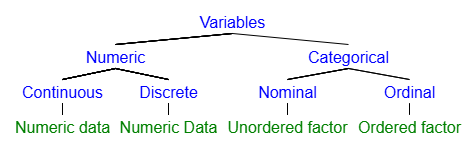
\includegraphics[keepaspectratio]{data_types.png}}

}

\caption{A hierarchy of variables and their corresponding R data types}

\end{figure}%

For our last bit, let's learn a little about working with functions that
don't come included in base R.

\chapter{Packages and the Tidyverse}\label{packages-and-the-tidyverse}

R's open-source culture has encouraged a rich ecosystem of custom
functions designed by scientists and researchers in the R userbase.
These come in the form of `packages', which are suites of several
related functions. For example, there are packages for conducting
statistical tests, producing data visualizations, generating
publication-ready tables, and all manner of other tasks.

\section{Loading Packages}\label{loading-packages}

Let's try this out with one of the better known R packages--`tidyverse'.
This is actually a collection of several packages with a variety of
interrelated functions for `tidying', visualizing, and analyzing data.
We will focus on what we need from `tidyverse', but, if you're curious,
you can read more here: \url{https://www.tidyverse.org/}

If you're on a lab computer, this package may already be installed.
Let's check by running the following command:

\begin{Shaded}
\begin{Highlighting}[]
\FunctionTok{library}\NormalTok{(tidyverse)}
\end{Highlighting}
\end{Shaded}

If you receive an error when you run this, you likely do not have the
package installed on your system. This is also probably the case if you
are on your personal device and only recently acquired R.

If you got an error, run the following command:

\begin{Shaded}
\begin{Highlighting}[]
\FunctionTok{install.packages}\NormalTok{(}\StringTok{"tidyverse"}\NormalTok{)}
\end{Highlighting}
\end{Shaded}

With a few exceptions, you will always install new packages in this
fashion: install.packages(``package\_name'')

After it's done installing, go back and run the library(tidyverse)
command again. Note that you always need to do this for an added
package. Whether you've had it for a while or just installed it, you
need to load any outside package into your current session by placing
its name in the library() function.

\begin{Shaded}
\begin{Highlighting}[]
\FunctionTok{library}\NormalTok{(tidyverse)}
\end{Highlighting}
\end{Shaded}

\section{Bringing in our Data}\label{bringing-in-our-data}

Let's try bringing in a data frame to play with a few tidyverse
functions. We'll use the \texttt{load()} function to bring in a subset
of the General Social Survey, which contains a few variables from the
2022 survey wave. Run the following command and select the file
``our\_gss.rda''

\begin{Shaded}
\begin{Highlighting}[]
\FunctionTok{load}\NormalTok{(}\FunctionTok{file.choose}\NormalTok{())}
\end{Highlighting}
\end{Shaded}

The \texttt{file.choose()} function will open up a file-explorer window
that allows you to manually select an R data file to load in. We'll talk
about some other ways to import data files using R syntax next time.

Go ahead and take a look at the data frame. Each GSS survey wave has
about 600-700 variables in total, so I've plucked several and done a
little pre-processing to get us a subset to work with. All the variables
here have pretty straightforward names, but I'll note that
\texttt{realrinc} is a clear outlier there. This is short for `Real
respondent's income' and reflects the respondent's income reported in
exact dollar amounts. I'll put a summary here so you can take a look if
you're not following along with your own script.

\begin{Shaded}
\begin{Highlighting}[]
\FunctionTok{summary}\NormalTok{(our\_gss)}
\end{Highlighting}
\end{Shaded}

\begin{verbatim}
      year            id              age           race          sex      
 Min.   :2022   Min.   :   1.0   Min.   :18.00   white:2514   female:1897  
 1st Qu.:2022   1st Qu.: 886.8   1st Qu.:34.00   other: 412   male  :1627  
 Median :2022   Median :1772.5   Median :48.00   black: 565   NA's  :  20  
 Mean   :2022   Mean   :1772.5   Mean   :49.18   NA's :  53                
 3rd Qu.:2022   3rd Qu.:2658.2   3rd Qu.:64.00                             
 Max.   :2022   Max.   :3545.0   Max.   :89.00                             
                                 NA's   :208                               
    realrinc                                      partyid   
 Min.   :   204.5   independent (neither, no response):835  
 1st Qu.:  8691.2   strong democrat                   :595  
 Median : 18405.0   not very strong democrat          :451  
 Mean   : 27835.3   strong republican                 :431  
 3rd Qu.: 33742.5   independent, close to democrat    :400  
 Max.   :141848.3   (Other)                           :797  
 NA's   :1554       NA's                              : 35  
           happy     
 not too happy: 799  
 pretty happy :1942  
 very happy   : 779  
 NA's         :  24  
                     
                     
                     
\end{verbatim}

\section{Data Wrangling with
Tidyverse}\label{data-wrangling-with-tidyverse}

Let's use this subset to explore some tidyverse functionality. One of
the packages included in the tidyverse is \texttt{dplyr}, which includes
several functions for efficiently manipulating data frames in
preparation for analyses. We will encounter a number of these throughout
our time with R, but I want to briefly introduce a few key
\texttt{dplyr} functions and operations that we will dig into more next
time.

\subsection{select()}\label{select}

It happens quite often that we have a data frame containing far more
variables than we need for a given analysis. The \texttt{select()}
function allows us to quickly subset data frames according to the
variable columns we specify.

This function takes a data frame as its first input, and all following
inputs are the variable columns that you want to keep

\begin{Shaded}
\begin{Highlighting}[]
\NormalTok{sex\_inc }\OtherTok{\textless{}{-}} \FunctionTok{select}\NormalTok{(our\_gss, id, sex, realrinc)}
\end{Highlighting}
\end{Shaded}

You should now have an object that contains all 3,544 observations, but
includes only the 3 columns that we specified with \texttt{select()}.

\begin{Shaded}
\begin{Highlighting}[]
\FunctionTok{summary}\NormalTok{(sex\_inc)}
\end{Highlighting}
\end{Shaded}

\begin{verbatim}
       id             sex          realrinc       
 Min.   :   1.0   female:1897   Min.   :   204.5  
 1st Qu.: 886.8   male  :1627   1st Qu.:  8691.2  
 Median :1772.5   NA's  :  20   Median : 18405.0  
 Mean   :1772.5                 Mean   : 27835.3  
 3rd Qu.:2658.2                 3rd Qu.: 33742.5  
 Max.   :3545.0                 Max.   :141848.3  
                                NA's   :1554      
\end{verbatim}

\subsection{filter()}\label{filter}

\texttt{filter()} functions similarly except that, instead of
sub-setting by specific variables, it allows you to subset by specific
values. So, let's take the \texttt{sex\_inc} object we just created
above. We now have this subset of three variables---id, sex, and
income---but let's imagine we want to answer a question that's specific
to women.

In order to do that, we need to \emph{filter} the data to include only
observations where the value of the variable \texttt{sex} is `female'.

\begin{Shaded}
\begin{Highlighting}[]
\NormalTok{fem\_inc }\OtherTok{\textless{}{-}} \FunctionTok{filter}\NormalTok{(sex\_inc, sex}\SpecialCharTok{==}\StringTok{"female"}\NormalTok{)}
\end{Highlighting}
\end{Shaded}

Note that the \texttt{fem\_inc} object still has 3 variables, but there
are now roughly half the observations, suggesting that we have
successfully filtered out the male observations.

\begin{Shaded}
\begin{Highlighting}[]
\FunctionTok{summary}\NormalTok{(fem\_inc)}
\end{Highlighting}
\end{Shaded}

\begin{verbatim}
       id           sex          realrinc       
 Min.   :   1   female:1897   Min.   :   204.5  
 1st Qu.: 879   male  :   0   1st Qu.:  7668.8  
 Median :1783                 Median : 15337.5  
 Mean   :1772                 Mean   : 22702.1  
 3rd Qu.:2664                 3rd Qu.: 27607.5  
 Max.   :3544                 Max.   :141848.3  
                              NA's   :883       
\end{verbatim}

\subsection{summarize()}\label{summarize}

As the name suggests, \texttt{summarize()} allows us to quickly
summarize information across variables. It will give us a new data frame
that reflects the summaries that we ask for, which can be very useful
for quickly generating descriptive statistics. We will use this to get
the mean income value for our data frame.

\begin{Shaded}
\begin{Highlighting}[]
\NormalTok{mean\_inc }\OtherTok{\textless{}{-}} \FunctionTok{summarize}\NormalTok{(our\_gss, }\StringTok{"mean\_inc"}\OtherTok{=}\FunctionTok{mean}\NormalTok{(realrinc, }\AttributeTok{na.rm=}\ConstantTok{TRUE}\NormalTok{))}
\end{Highlighting}
\end{Shaded}

\begin{tcolorbox}[enhanced jigsaw, colframe=quarto-callout-note-color-frame, arc=.35mm, coltitle=black, breakable, rightrule=.15mm, left=2mm, opacitybacktitle=0.6, colbacktitle=quarto-callout-note-color!10!white, toptitle=1mm, bottomtitle=1mm, titlerule=0mm, leftrule=.75mm, colback=white, title=\textcolor{quarto-callout-note-color}{\faInfo}\hspace{0.5em}{Note}, opacityback=0, bottomrule=.15mm, toprule=.15mm]

You probably noticed the \texttt{na.rm\ =\ TRUE} input that I supplied
for the above function. This is short for `remove NAs', which we need to
do when a variable has any NA values. If we don't, R will screw up,
because it does not know to disregard NA values when calculating a
column mean unless we tell it to.

\end{tcolorbox}

This gives us a new data frame that we called \texttt{mean\_inc}. It
should have 1 row and 1 column, and it just gives us the average income
of a person in our GSS subset---about \$28,000/year.

\begin{Shaded}
\begin{Highlighting}[]
\NormalTok{mean\_inc}
\end{Highlighting}
\end{Shaded}

\begin{verbatim}
  mean_inc
1 27835.33
\end{verbatim}

Now, this is not really all that impressive when we are asking for a
broad summary like this. In fact, if all we wanted was to see the
average income, we could get that more easily, e.g.

\begin{Shaded}
\begin{Highlighting}[]
\FunctionTok{mean}\NormalTok{(our\_gss}\SpecialCharTok{$}\NormalTok{realrinc, }\AttributeTok{na.rm =} \ConstantTok{TRUE}\NormalTok{)}
\end{Highlighting}
\end{Shaded}

\begin{verbatim}
[1] 27835.33
\end{verbatim}

The true power of \texttt{summarize()} comes from chaining it together
with other tidyverse functions. However, in order to do that, we will
need to learn about one more new R operation. I'll show you that in a
moment, but let's take a look at one more helpful tidyverse function.

\subsection{group\_by()}\label{group_by}

Often when we're using a function like \texttt{summarize()}, we want to
get summaries for all kinds of different subgroups within our data set.
For example, we may want the mean for each value of \texttt{sex} or
\texttt{partyid}, rather than for all people in the data frame. We can
do this with \texttt{group\_by}.

This function may seem a little unusual when used in isolation, because
it does not seem to do much on the surface.

\begin{Shaded}
\begin{Highlighting}[]
\NormalTok{our\_gss }\OtherTok{\textless{}{-}} \FunctionTok{group\_by}\NormalTok{(our\_gss, partyid)}
\end{Highlighting}
\end{Shaded}

When you run that function, you will not generate any new objects, and
you will not notice anything different about the data frame.

What it does is overlay a grouping structure on the data frame, which
will in turn affect how other tidyverse functions operate.

Compare the output of \texttt{summarize()} run on this grouped version
of our data frame with the use of \texttt{summarize()} above.

\begin{Shaded}
\begin{Highlighting}[]
\NormalTok{mean\_inc }\OtherTok{\textless{}{-}} \FunctionTok{summarize}\NormalTok{(}
\NormalTok{  our\_gss,}
  \StringTok{"mean\_inc"} \OtherTok{=} \FunctionTok{mean}\NormalTok{(realrinc, }\AttributeTok{na.rm =} \ConstantTok{TRUE}\NormalTok{)}
\NormalTok{  )}

\NormalTok{mean\_inc}
\end{Highlighting}
\end{Shaded}

\begin{verbatim}
# A tibble: 9 x 2
  partyid                            mean_inc
  <fct>                                 <dbl>
1 strong democrat                      30677.
2 independent (neither, no response)   21570.
3 not very strong republican           29101.
4 not very strong democrat             31743.
5 independent, close to democrat       27916.
6 other party                          23891.
7 independent, close to republican     26825.
8 strong republican                    32376.
9 <NA>                                 16922.
\end{verbatim}

We ran the same \texttt{summarize()} command as before, but now it
reflects the grouping structure that we imposed.

\section{The Pipe}\label{the-pipe}

This one might be a little unintuitive, so don't worry if it doesn't
immediately click. We will continue to get plenty of practice with it
over the next couple of sessions.

The pipe operator looks like this: \texttt{\textbar{}\textgreater{}}.
What it does is take whatever is to the left of the symbol and `pipe' it
into the function on the right-hand side. That probably sounds a little
strange, so let's see some examples.

We'll refer back to our \texttt{summarize()} command from above.

\begin{Shaded}
\begin{Highlighting}[]
\NormalTok{mean\_inc }\OtherTok{\textless{}{-}} \FunctionTok{summarize}\NormalTok{(our\_gss, }\StringTok{"mean\_inc"}\OtherTok{=}\FunctionTok{mean}\NormalTok{(realrinc, }\AttributeTok{na.rm=}\ConstantTok{TRUE}\NormalTok{))}
\end{Highlighting}
\end{Shaded}

This is equivalent to\ldots{}

\begin{Shaded}
\begin{Highlighting}[]
\NormalTok{mean\_inc }\OtherTok{\textless{}{-}}\NormalTok{ our\_gss }\SpecialCharTok{|\textgreater{}}
  \FunctionTok{summarize}\NormalTok{(}\StringTok{"mean\_age"} \OtherTok{=} \FunctionTok{mean}\NormalTok{(realrinc, }\AttributeTok{na.rm=}\ConstantTok{TRUE}\NormalTok{))}
\end{Highlighting}
\end{Shaded}

Notice that, in the first command, the first input that we give
\texttt{summarize()} is the data frame that we want it to work with.

In the command featuring the pipe operator, we supply the data frame and
then pipe it into \texttt{summarize()}. The real magic comes from
chaining multiple pipes together. This will likely take a little
practice to get used to, but it can become a very powerful tool in our R
arsenal.

\subsection{Putting It All Together}\label{putting-it-all-together}

Let's illustrate with an example. I'll let you know what I want to do in
plain English, and then I will execute that desire with multiple piped
commands.

Ultimately, I want to see the mean income, but I want to see the mean
broken down by \texttt{sex} and \texttt{partyid.}

So, I want to take a \textbf{selection} of variables from
\texttt{our\_gss}. I want these variables to be \textbf{grouped by}
\texttt{sex} and \texttt{partyid}. Finally, I want to see a
\textbf{summary} of the mean according to this variable grouping.

\begin{Shaded}
\begin{Highlighting}[]
\NormalTok{sexpol\_means }\OtherTok{\textless{}{-}}\NormalTok{ our\_gss }\SpecialCharTok{|\textgreater{}}
  \FunctionTok{select}\NormalTok{(id, sex, realrinc, partyid) }\SpecialCharTok{|\textgreater{}}
  \FunctionTok{group\_by}\NormalTok{(sex, partyid) }\SpecialCharTok{|\textgreater{}}
  \FunctionTok{summarize}\NormalTok{(}\StringTok{"mean\_inc"} \OtherTok{=} \FunctionTok{mean}\NormalTok{(realrinc, }\AttributeTok{na.rm=}\ConstantTok{TRUE}\NormalTok{)) }\SpecialCharTok{|\textgreater{}}
  \FunctionTok{drop\_na}\NormalTok{(sex, partyid)}
\end{Highlighting}
\end{Shaded}

\begin{verbatim}
`summarise()` has grouped output by 'sex'. You can override using the `.groups`
argument.
\end{verbatim}

\begin{tcolorbox}[enhanced jigsaw, colframe=quarto-callout-note-color-frame, arc=.35mm, coltitle=black, breakable, rightrule=.15mm, left=2mm, opacitybacktitle=0.6, colbacktitle=quarto-callout-note-color!10!white, toptitle=1mm, bottomtitle=1mm, titlerule=0mm, leftrule=.75mm, colback=white, title=\textcolor{quarto-callout-note-color}{\faInfo}\hspace{0.5em}{Note}, opacityback=0, bottomrule=.15mm, toprule=.15mm]

We can use \texttt{drop\_na()} to do as the function's name suggests.
When we learned about \texttt{group\_by()} above, you may have noticed
that a mean was reported for an \texttt{NA} category within the
\texttt{partyid} variable. Any time you notice this and want your
summaries to exclude these NA categories, just include that variable as
an input to \texttt{drop\_na()}.

\end{tcolorbox}

\begin{Shaded}
\begin{Highlighting}[]
\NormalTok{sexpol\_means}
\end{Highlighting}
\end{Shaded}

\begin{verbatim}
# A tibble: 16 x 3
# Groups:   sex [2]
   sex    partyid                            mean_inc
   <fct>  <fct>                                 <dbl>
 1 female strong democrat                      30111.
 2 female independent (neither, no response)   17923.
 3 female not very strong republican           22448.
 4 female not very strong democrat             24300.
 5 female independent, close to democrat       19961.
 6 female other party                          26595.
 7 female independent, close to republican     20095.
 8 female strong republican                    21584.
 9 male   strong democrat                      31600.
10 male   independent (neither, no response)   25474.
11 male   not very strong republican           34544.
12 male   not very strong democrat             41233.
13 male   independent, close to democrat       36947.
14 male   other party                          22450.
15 male   independent, close to republican     31393.
16 male   strong republican                    40210.
\end{verbatim}

So, using \texttt{dplyr}, we can quickly subset and manipulate data
frames in just a few lines of relatively straightforward code. Here we
have all the means for each value of \texttt{sex} and \texttt{partyid},
which would have been a tedious task had we calculated them all
manually.

We will see plenty more on the tidyverse, so don't fret if you don't
feel completely confident with these yet. It takes practice getting used
to Rs peculiarities. We will keep building with these in the next unit
and hopefully accumulate some muscle memory.

\part{Day 2: Survey Data and Univariate Analysis}

\chapter{Recoding Variables}\label{recoding-variables}

Today's venture concerns univariate analysis, i.e.~the quantitative
description of a single variable. Before we do that, however, we need to
familiarize ourselves with some data-cleaning procedures.

\section{Background}\label{background-1}

Recoding a variable involves manipulating the underlying structure of
our variable such that we can use it for analysis. We did a little
recoding during the last unit when we converted character vectors into
factor variables. This allowed us to align R data types with the
appropriate level of measurement.

There are also occasions when we need a variable to be translated from
one level of measurement to another. For example, we may want to convert
a ratio variable for ``number of years of education'' into an ordinal
variable reflecting categories like ``less than high school'', ``high
school diploma'', ``Associates degree'', and so on.

We may also want to collapse the categories of ordinal variables for
some analyses. Consider a variable with a Likert-scale agreement rating,
where you responses like ``strongly agree,'' ``moderately agree,''
``slightly agree,'' and so forth. You may decide to collapse these
categories into categories of ``Agree'' and ``Disagree''.

We will get some practice doing this sort of thing, which is an
essential component of responsible analysis. Additionally, our next unit
on bivariate analysis will require us to work with categorical variables
in particular, so we need to be capable of converting any numeric
variables.

\section{Converting Numeric to
Categorical}\label{converting-numeric-to-categorical}

We will start by recoding \texttt{age}---a ratio variable---into an
ordinal variable reflecting age groupings. The same strategies we use
here will work for any numeric variable.

\subsection{Setting up our workspace}\label{setting-up-our-workspace}

As usual, let's make sure we load in \texttt{tidyverse} along with our
GSS data.

\begin{Shaded}
\begin{Highlighting}[]
\FunctionTok{library}\NormalTok{(tidyverse)}
\FunctionTok{load}\NormalTok{(}\StringTok{"our\_gss.rda"}\NormalTok{)}
\end{Highlighting}
\end{Shaded}

Let's double check the structure of our data frame.

\begin{Shaded}
\begin{Highlighting}[]
\FunctionTok{str}\NormalTok{(our\_gss)}
\end{Highlighting}
\end{Shaded}

\begin{verbatim}
'data.frame':   3544 obs. of  8 variables:
 $ year    : int  2022 2022 2022 2022 2022 2022 2022 2022 2022 2022 ...
 $ id      : int  1 2 3 4 5 6 7 8 9 10 ...
 $ age     : int  72 80 57 23 62 27 20 47 31 72 ...
 $ race    : Factor w/ 3 levels "white","other",..: 1 1 1 1 1 1 2 1 1 NA ...
 $ sex     : Factor w/ 2 levels "female","male": 1 2 1 1 2 2 1 2 1 1 ...
 $ realrinc: num  40900 NA 18405 2250 NA ...
 $ partyid : Factor w/ 8 levels "strong democrat",..: 1 2 3 1 2 4 5 1 5 1 ...
 $ happy   : Ord.factor w/ 3 levels "not too happy"<..: 1 1 1 1 2 2 2 2 2 2 ...
\end{verbatim}

\begin{tcolorbox}[enhanced jigsaw, colframe=quarto-callout-note-color-frame, arc=.35mm, coltitle=black, breakable, rightrule=.15mm, left=2mm, opacitybacktitle=0.6, colbacktitle=quarto-callout-note-color!10!white, toptitle=1mm, bottomtitle=1mm, titlerule=0mm, leftrule=.75mm, colback=white, title=\textcolor{quarto-callout-note-color}{\faInfo}\hspace{0.5em}{Note}, opacityback=0, bottomrule=.15mm, toprule=.15mm]

You might notice the `int' category, which is short for `integer'. This
is a subtype of numeric data in R. Variables that are exclusively whole
numbers are often recorded in this way, but we can work with them in R
just like we can other sorts of numbers

\end{tcolorbox}

\subsection{The `age' variable}\label{the-age-variable}

We can take a look at all the values of age (along with the \# of
respondents in each age category) using the \texttt{count()} function.

\begin{Shaded}
\begin{Highlighting}[]
\FunctionTok{count}\NormalTok{(our\_gss, age)}
\end{Highlighting}
\end{Shaded}

However, I'm not going to display those results here, as it will be a
particularly long table of values (with 70+ different ages). It's fine
to run it---it won't crash R or anything---but it will it clutter up
this page. Let's take this as a good opportunity to take advantage of
the fact that we are using one of the better funded and well-organized
surveys in all of social sciences. As such, there's extensive
documentation about all of the variables measured for the GSS.
\href{https://gssdataexplorer.norc.org/variables/53/vshow}{Go ahead and
take a look at the age variable via the GSS Data Explorer}, which allows
us to search for unique variables and view their response values, the
specific question(s) that was asked on the survey, and several other
variable characteristics.

The responses range from 18 - 89 (in addition to a few categories for
non-response). However, note that there's something unique about value
89. It's not just 89 years of age, but 89 \& older. This isn't a real
issue for our purposes, but take this as encouragement to interface with
the codebook of any publicly available data you use. There's some
imprecision at the upper end of this variable, and that might not be
obvious without referencing the codebook.

For the purposes of this exercise, let's go ahead and turn age into a
simple categorical variable with 3 levels---older, middle age, and
younger. I'm going to choose the range somewhat arbitrarily for now. We
can use univariate analysis to inform our decision about how to break up
a numeric variable, so we will revisit this idea again later on.

\begin{itemize}
\tightlist
\item
  \textbf{Younger} = 18 - 35
\item
  \textbf{Middle Age} = 36 - 49
\item
  \textbf{Older} = 50 and up
\end{itemize}

At the end of the day, what we need to do is 1.) create a new variable
column 2.) populate that column with ordinal labels that correspond with
each respondent's numeric age interval.

\subsection{New columns with mutate()}\label{new-columns-with-mutate}

First, let's consider the \texttt{mutate()} function. This function
takes a data frame and appends a new variable column. This new variable
is the result of some calculation applied to an existing variable
column.

Let's look at an application fo \texttt{mutate()} to get a feel for it.
Now, this wouldn't be the best idea for a couple reasons, but, as an
illustration, let's say we wanted to convert our yearly income values to
an hourly wage (assuming 40 hrs/week).

\texttt{mutate()} takes a data frame as its input, and then we provide
the name of our new variable column(s) along with the calculation for
this new variable. Below, I use \texttt{mutate()} to create a new column
called \texttt{hr\_wage}. Then, I tell R that the \texttt{hr\_wage}
variable should be calculated by taking each person's income value and
diving that by 52 weeks in a year, and then 40 hours in a week.

\begin{Shaded}
\begin{Highlighting}[]
\CommentTok{\# Without the pipe operator}
\NormalTok{our\_gss }\OtherTok{\textless{}{-}} \FunctionTok{mutate}\NormalTok{(}
\NormalTok{  our\_gss,}
  \AttributeTok{hr\_wage =}\NormalTok{ (realrinc}\SpecialCharTok{/}\DecValTok{52}\NormalTok{)}\SpecialCharTok{/}\DecValTok{40}
\NormalTok{  )}
\end{Highlighting}
\end{Shaded}

\begin{Shaded}
\begin{Highlighting}[]
\CommentTok{\# With the pipe operator}
\NormalTok{our\_gss }\OtherTok{\textless{}{-}}\NormalTok{ our\_gss }\SpecialCharTok{|\textgreater{}}
  \FunctionTok{mutate}\NormalTok{(}
    \AttributeTok{hr\_wage =}\NormalTok{ (realrinc}\SpecialCharTok{/}\DecValTok{52}\NormalTok{)}\SpecialCharTok{/}\DecValTok{40}
\NormalTok{  )}
\end{Highlighting}
\end{Shaded}

Take a look at your new data frame object. I'll show a summary here to
verify that we got our new column.

\begin{Shaded}
\begin{Highlighting}[]
\FunctionTok{summary}\NormalTok{(our\_gss)}
\end{Highlighting}
\end{Shaded}

\begin{verbatim}
      year            id              age           race          sex      
 Min.   :2022   Min.   :   1.0   Min.   :18.00   white:2514   female:1897  
 1st Qu.:2022   1st Qu.: 886.8   1st Qu.:34.00   other: 412   male  :1627  
 Median :2022   Median :1772.5   Median :48.00   black: 565   NA's  :  20  
 Mean   :2022   Mean   :1772.5   Mean   :49.18   NA's :  53                
 3rd Qu.:2022   3rd Qu.:2658.2   3rd Qu.:64.00                             
 Max.   :2022   Max.   :3545.0   Max.   :89.00                             
                                 NA's   :208                               
    realrinc                                      partyid   
 Min.   :   204.5   independent (neither, no response):835  
 1st Qu.:  8691.2   strong democrat                   :595  
 Median : 18405.0   not very strong democrat          :451  
 Mean   : 27835.3   strong republican                 :431  
 3rd Qu.: 33742.5   independent, close to democrat    :400  
 Max.   :141848.3   (Other)                           :797  
 NA's   :1554       NA's                              : 35  
           happy         hr_wage        
 not too happy: 799   Min.   : 0.09832  
 pretty happy :1942   1st Qu.: 4.17849  
 very happy   : 779   Median : 8.84856  
 NA's         :  24   Mean   :13.38237  
                      3rd Qu.:16.22236  
                      Max.   :68.19631  
                      NA's   :1554      
\end{verbatim}

So, we can use \texttt{mutate()} to add a new column that contains our
recoded variable. We just need a way to specify a calculation that takes
into account the specific intervals we want for our ordinal labels. For
this, we need one more function.

\subsection{Custom intervals with
cut()}\label{custom-intervals-with-cut}

We can use the \texttt{cut()} function to specify the intervals we want
for our age groupings, and then we will combine it with
\texttt{mutate()} to generate our recoded age variable. Specifically,
\texttt{cut()} takes our intervals and turns each of them into a level
in a new factor variable.

But first, I want to give a little context on interval notation in
mathematics. It will help us all be a little more precise when we talk
about ranges, and it will also help us understand an input we need to
provide for \texttt{cut()}.

\subsubsection{An aside on intervals}\label{an-aside-on-intervals}

In mathematic terms, an interval is the set of all numbers in between
two specified end points. In formal notation, these are indicated with
the two endpoints placed in square brackets, e.g {[}1,5{]} as the
interval of 1 through 5.

There are some technical terms to describe whether or not we want to
include the endpoints when we are talking about a particular interval.

\begin{itemize}
\item
  \textbf{Closed interval}: This is when both end points are included in
  the interval. Closedness is indicated with square brackets, so, the
  closed interval of 1 through 5 would be written just like I have
  above---{[}1,5{]}. This indicates any number `x' where 1 \textless= x
  \textless= 5
\item
  \textbf{Open interval}: This is when neither endpoint is included in
  the interval. In interval notation, openness is indicated with
  parentheses rather than square brackets, so the open interval of 1
  through 5 would be written as (1,5). This interval would indicate any
  number `x' where 1 \textless{} x \textless{} 5
\item
  \textbf{Left-open interval}: This is when the left-hand endpoint is
  not included, but the right-hand endpoint is. This would be written as
  (1,5{]} in interval notation, and that interval would indicate any
  number `x' where 1 \textless{} x \textless= 5
\item
  \textbf{Right-open interval}: When the right-hand endpoint isn't
  included but the left endpoint is, you have a right-open interval.
  This would be written as {[}1,5) in interval notation and would
  indicate any number `x' where 1 \textless= x \textless{} 5.
\end{itemize}

We will be working with the right-open interval format, and we can
specify that in \texttt{cut()}.

Now, let's return to our task at hand.

\subsubsection{Inputs for cut()}\label{inputs-for-cut}

We'll go ahead and work with cut directly in \texttt{mutate()}, as its
going to be the calculation that we are providing for the new column we
generate with \texttt{mutate()}.

As a reminder, here are the intervals we need:

\begin{itemize}
\tightlist
\item
  \textbf{Younger} = 18 - 35
\item
  \textbf{Middle Age} = 36 - 49
\item
  \textbf{Older} = 50 and up
\end{itemize}

The following code may look a little chaotic at first glance, but it's
really the same sort of thing that we did with \texttt{mutate()} above.
It's just that \texttt{cut()} is a little bit more involved of a
calculation than the simple division we did in our example.

Just like above, we are applying \texttt{mutate()} to \texttt{our\_gss},
and we are giving the name of our new variable column
(\texttt{age\_ord}, in this case) as the first input. Then, for the
calculation, we give the \texttt{cut()} function and the arguments it
needs.

\textbf{cut() and its inputs}

\begin{itemize}
\item
  The variable for which we want to specify intervals (\texttt{age})
\item
  \textbf{breaks}: This is where we indicate the intervals. The first
  number we give is the low end of our lowest age group (18). The second
  number is the low end of our middle age group (36). The third number,
  as you probably guessed, is the low end of our highest age group. The
  last value should reflect our upper limit. In this case, I use the
  value \texttt{Inf}, which is short for `infinity'. This essentially
  tells R that the last category can include any values higher than the
  previous number we entered.
\item
  \textbf{include.lowest}: Putting \texttt{TRUE} here tells R that, in
  each interval, we want the lowest value to be included. If we don't do
  this, then our `younger' age grouping would be 19 - 35 rather than 18
  - 35. In other words, setting this to \texttt{TRUE} indicates a
  left-closed interval, and \texttt{FALSE} indicates a left-open
  interval.
\item
  \textbf{right}: This is the input for specifying whether we want this
  to be a right-closed interval, and it takes a logical value
  (\texttt{TRUE} or \texttt{FALSE}). We want a right-open interval, so
  we will set this to \texttt{FALSE}.
\item
  \textbf{labels}: R will actually default to formal interval notation
  for the names of each level of our new factor variable, so it would be
  {[}18,36), {[}36,50), {[}50, Inf). However, we can provide a character
  vector to specify custom labels for these new factor levels. In the
  event that you have an ordinal variable, make sure that you always
  specify these labels in ascending order. In this case, that would be
  Younger \textless{} Middle Age \textless{} Older.
\item
  \textbf{ordered\_result}: This takes a logical value and, as the name
  suggests, indicates whether we want the factor to be ordered or not.
  In our case, there is a clear progression in terms of age, so we need
  to set this to \texttt{TRUE}.
\end{itemize}

\begin{Shaded}
\begin{Highlighting}[]
\NormalTok{our\_gss }\OtherTok{\textless{}{-}}\NormalTok{ our\_gss }\SpecialCharTok{|\textgreater{}}
  \FunctionTok{mutate}\NormalTok{(}
    \AttributeTok{age\_ord =} \FunctionTok{cut}\NormalTok{(}
\NormalTok{      age,}
      \AttributeTok{breaks =} \FunctionTok{c}\NormalTok{(}\DecValTok{18}\NormalTok{, }\DecValTok{36}\NormalTok{, }\DecValTok{51}\NormalTok{, }\ConstantTok{Inf}\NormalTok{),}
      \AttributeTok{include.lowest =} \ConstantTok{TRUE}\NormalTok{,}
      \AttributeTok{right =} \ConstantTok{FALSE}\NormalTok{,}
      \AttributeTok{labels =} \FunctionTok{c}\NormalTok{(}\StringTok{"Younger"}\NormalTok{, }\StringTok{"Middle Age"}\NormalTok{, }\StringTok{"Older"}\NormalTok{),}
      \AttributeTok{ordered\_result =} \ConstantTok{TRUE}
\NormalTok{    )}
\NormalTok{  )}
\end{Highlighting}
\end{Shaded}

Go ahead and take a look at \texttt{our\_gss}, and our new column should
bring us to 10 variables instead of 9. I'll use the \texttt{str()}
function here so we can confirm that our factor was ordered and added to
the data frame.

\begin{Shaded}
\begin{Highlighting}[]
\FunctionTok{str}\NormalTok{(our\_gss)}
\end{Highlighting}
\end{Shaded}

\begin{verbatim}
'data.frame':   3544 obs. of  10 variables:
 $ year    : int  2022 2022 2022 2022 2022 2022 2022 2022 2022 2022 ...
 $ id      : int  1 2 3 4 5 6 7 8 9 10 ...
 $ age     : int  72 80 57 23 62 27 20 47 31 72 ...
 $ race    : Factor w/ 3 levels "white","other",..: 1 1 1 1 1 1 2 1 1 NA ...
 $ sex     : Factor w/ 2 levels "female","male": 1 2 1 1 2 2 1 2 1 1 ...
 $ realrinc: num  40900 NA 18405 2250 NA ...
 $ partyid : Factor w/ 8 levels "strong democrat",..: 1 2 3 1 2 4 5 1 5 1 ...
 $ happy   : Ord.factor w/ 3 levels "not too happy"<..: 1 1 1 1 2 2 2 2 2 2 ...
 $ hr_wage : num  19.66 NA 8.85 1.08 NA ...
 $ age_ord : Ord.factor w/ 3 levels "Younger"<"Middle Age"<..: 3 3 3 1 3 1 1 2 1 3 ...
\end{verbatim}

\section{Restructuring Categorical
Variables}\label{restructuring-categorical-variables}

Now, let's go ahead and tackle the other recoding situation I mentioned
up at the top---collapsing the levels of categorical variables. We'll
work with \texttt{partyid} here, but the logic of this process will
apply to any categorical variable.

\subsection{Collapsing categories}\label{collapsing-categories}

I encourage you to take a look at \texttt{partyid} in
\href{https://gssdataexplorer.norc.org/variables/141/vshow}{the GSS Data
Explorer, like we did for `age'.}.

Because \texttt{partyid} is a categorical variable, it has far fewer
unique values than a ratio variable like \texttt{age}, so we can go
ahead and take a look at all of its levels with the \texttt{count()}
function.

\begin{tcolorbox}[enhanced jigsaw, colframe=quarto-callout-note-color-frame, arc=.35mm, coltitle=black, breakable, rightrule=.15mm, left=2mm, opacitybacktitle=0.6, colbacktitle=quarto-callout-note-color!10!white, toptitle=1mm, bottomtitle=1mm, titlerule=0mm, leftrule=.75mm, colback=white, title=\textcolor{quarto-callout-note-color}{\faInfo}\hspace{0.5em}{Note}, opacityback=0, bottomrule=.15mm, toprule=.15mm]

Observe that \texttt{count(our\_gss,\ partyid)} basically provides the
same information as \texttt{summary(our\_gss\$partyid)} when the
variable is a factor. The only real difference is that \texttt{count()}
organizes the info into a tidy data frame. In other words, you can use
either function to take a look at factor variable like this.

\end{tcolorbox}

\begin{Shaded}
\begin{Highlighting}[]
\FunctionTok{count}\NormalTok{(our\_gss, partyid)}
\end{Highlighting}
\end{Shaded}

\begin{verbatim}
                             partyid   n
1                    strong democrat 595
2 independent (neither, no response) 835
3         not very strong republican 361
4           not very strong democrat 451
5     independent, close to democrat 400
6                        other party 106
7   independent, close to republican 330
8                  strong republican 431
9                               <NA>  35
\end{verbatim}

Let's go ahead and collapse these into categories of ``Democrat'',
``Independent'', ``Other Party'', and ``Republican''. We'll use
\texttt{mutate()} to make a new variable column called
\texttt{partyid\_recoded}. For the calculation of our new variable, we
can use the \texttt{fct\_collapse()} function. This function allows us
to first give the name of a new factor level, and then we can give a
character vector of the names of levels that want to be collapses into a
single category.

So, to collapse our 3 Democrat levels into a single factor level, we
would give the following input for \texttt{fct\_collapse()}:

\texttt{"Democrat"\ =\ c("strong\ democrat",\ "not\ very\ strong\ democrat")}

And then repeat for each new factor level.

\begin{Shaded}
\begin{Highlighting}[]
\NormalTok{our\_gss }\OtherTok{\textless{}{-}}\NormalTok{ our\_gss }\SpecialCharTok{|\textgreater{}}
  \FunctionTok{mutate}\NormalTok{(}
    \AttributeTok{partyid\_recoded=}\FunctionTok{fct\_collapse}\NormalTok{(partyid, }
\StringTok{"Democrat"} \OtherTok{=} \FunctionTok{c}\NormalTok{(}\StringTok{"strong democrat"}\NormalTok{, }\StringTok{"not very strong democrat"}\NormalTok{),}
\StringTok{"Republican"} \OtherTok{=} \FunctionTok{c}\NormalTok{(}\StringTok{"strong republican"}\NormalTok{,}\StringTok{"not very strong republican"}\NormalTok{),}
\StringTok{"Independent"} \OtherTok{=} \FunctionTok{c}\NormalTok{(}\StringTok{"independent, close to democrat"}\NormalTok{, }\StringTok{"independent (neither, no response)"}\NormalTok{, }\StringTok{"independent, close to republican"}\NormalTok{),}
\StringTok{"Other Party"} \OtherTok{=} \FunctionTok{c}\NormalTok{(}\StringTok{"other party"}\NormalTok{)}
\NormalTok{))}
\end{Highlighting}
\end{Shaded}

Now, let's take a look at our new variable.

\begin{Shaded}
\begin{Highlighting}[]
\FunctionTok{count}\NormalTok{(our\_gss, partyid\_recoded)}
\end{Highlighting}
\end{Shaded}

\begin{verbatim}
  partyid_recoded    n
1        Democrat 1046
2     Independent 1565
3      Republican  792
4     Other Party  106
5            <NA>   35
\end{verbatim}

\subsection{Excluding levels}\label{excluding-levels}

You may also want to work with an existing categorical variable, but
only focus on certain values. In this case, we can create a recoded
variable and simply code the levels we are uninterested in as
\texttt{NA}.

We can use the \texttt{fct\_recode()} function for this. For the first
input, we will give it the factor-variable column that we want to
recode. Then, we will let it know that we want to set the levels of
``Other Party'' and ``Independent'' to \texttt{NULL}. This will convert
them to NAs and allow us to easily exclude them from our analyses. We
will use \texttt{fct\_recode()} within \texttt{mutate()} so we can
create another recoded version of \texttt{partyid\_recoded}. We'll call
this one \texttt{dem\_rep} to distinguish it from the original
\texttt{partyid} and our first recoded version.

\begin{Shaded}
\begin{Highlighting}[]
\NormalTok{our\_gss }\OtherTok{\textless{}{-}}\NormalTok{ our\_gss }\SpecialCharTok{|\textgreater{}}
  \FunctionTok{mutate}\NormalTok{(}\AttributeTok{dem\_rep =} \FunctionTok{fct\_recode}\NormalTok{(}
\NormalTok{    partyid\_recoded, }
    \AttributeTok{NULL=}\StringTok{"Other Party"}\NormalTok{, }
    \AttributeTok{NULL=}\StringTok{"Independent"}\NormalTok{))}
\end{Highlighting}
\end{Shaded}

Let's check to see that it worked.

\begin{Shaded}
\begin{Highlighting}[]
\FunctionTok{count}\NormalTok{(our\_gss, dem\_rep)}
\end{Highlighting}
\end{Shaded}

\begin{verbatim}
     dem_rep    n
1   Democrat 1046
2 Republican  792
3       <NA> 1706
\end{verbatim}

Now that we have gotten all this pre-processing stuff out of the way,
let's go ahead and dig into some univariate analysis.

\chapter{Univariate: Categorical}\label{univariate-categorical}

Before we start examining the relationships between multiple variables,
we have to look under the hood of our variables individually and make
sure we have a good sense of what they are like.

We want to know the frequency distribution of the response values, the
measures of central tendency, and the dispersion. In other words, we
want to see how many respondents chose each response value, which
response values are most typical for each variable, and the extent to
which the response values vary.

Luckily for us, R has plenty of tools for generating these quantitative
summaries, as well as visualizing them in the form of barplots,
histograms, and other common styles for displaying data.

This tutorial will cover each of these elements, and I will highlight
any differences specific to certain levels of measurement along the way.

\section{Frequency Distributions}\label{frequency-distributions}

Let's start with categorical variables. We will start with frequency
distributions by way of frequency tables and bar plots. Then, we will
talk about measures of tendency and observe when they are appropriate
for categorical data.

\subsection{Frequency tables}\label{frequency-tables}

Frequency tables are the most effective way to report the frequency
distributions for categorical variables. There are actually a ton of
different ways to produce this kind of table in R, but we are going to
use some convenient functions from the \texttt{janitor} package, so
let's go ahead and load that in.

If you are on a lab computer, try to load it with \texttt{library()}
first. If you get an error, go ahead and install it with
\texttt{install.packages()} and then load it in.

While we're at it, we'll also bring in \texttt{tidyverse} and load in
our GSS subset.

\begin{Shaded}
\begin{Highlighting}[]
\FunctionTok{library}\NormalTok{(janitor)}
\FunctionTok{library}\NormalTok{(tidyverse)}
\FunctionTok{load}\NormalTok{(}\StringTok{"our\_gss.rda"}\NormalTok{)}
\end{Highlighting}
\end{Shaded}

Let's go ahead and work with one of our \texttt{partyid} recodes from
last time. We'll use \texttt{partyid\_recoded}, where we retained all
the party choices but collapsed the categories of degree (e.g.~strong
democrat + not very strong democrat = Democrat).

We can use a simple command with \texttt{tabyl()} from the
\texttt{janitor} package to produce our frequency tables. Let's take a
look at some output, and I'll go through a couple details and mention
some further specifications we can make.

All we need to do is give our data frame as the first argument, and then
our particular variable column as the second argument.

\begin{Shaded}
\begin{Highlighting}[]
\CommentTok{\# Without pipe operator}
\FunctionTok{tabyl}\NormalTok{(our\_gss, partyid\_recoded)}
\end{Highlighting}
\end{Shaded}

\begin{Shaded}
\begin{Highlighting}[]
\CommentTok{\# With pipe operator}
\NormalTok{our\_gss }\SpecialCharTok{|\textgreater{}}
  \FunctionTok{tabyl}\NormalTok{(partyid\_recoded)}
\end{Highlighting}
\end{Shaded}

\begin{verbatim}
 partyid_recoded    n     percent valid_percent
        Democrat 1046 0.295146727    0.29809062
     Independent 1565 0.441591422    0.44599601
      Republican  792 0.223476298    0.22570533
     Other Party  106 0.029909707    0.03020804
            <NA>   35 0.009875847            NA
\end{verbatim}

Now, we have a frequency table for \texttt{partyid\_recoded}!

Each row is a level of \texttt{partyid\_recoded}. The \texttt{n} column
refers to the sample size, so, for example, 1,565 respondents indicated
that they were Independents.

We then have two different columns for percentages. The \texttt{percent}
column is the proportion of all respondents that chose each response
value---while including NA values. Often, we want to get a proportion
for only the sample of those who actually answered the question. This is
what the \texttt{valid\_percent} column indicates and is what we are
often looking for.

Let's break it down a little for clarity.

The total number of respondents is the sum of the `n' column.

1565 + 1046 + 792 + 106 + 35 = 3,544

Note that this is also the number of observations in our data frame

There are also 35 observations coded as NA, so the total number of
\emph{valid} respondents is 3,509.

Now, I'll give the calculations for the \texttt{Independent} row.

\begin{Shaded}
\begin{Highlighting}[]
\CommentTok{\# I\textquotesingle{}m going to define a few objects here for simplicity.}

\NormalTok{all\_respondents }\OtherTok{\textless{}{-}} \DecValTok{3544}

\NormalTok{all\_minus\_na }\OtherTok{\textless{}{-}}\NormalTok{ (}\DecValTok{3544} \SpecialCharTok{{-}} \DecValTok{35}\NormalTok{)}

\NormalTok{independents }\OtherTok{\textless{}{-}} \DecValTok{1565}
\end{Highlighting}
\end{Shaded}

\begin{Shaded}
\begin{Highlighting}[]
\CommentTok{\# Percent column}

\NormalTok{independents }\SpecialCharTok{/}\NormalTok{ all\_respondents}
\end{Highlighting}
\end{Shaded}

\begin{verbatim}
[1] 0.4415914
\end{verbatim}

\begin{Shaded}
\begin{Highlighting}[]
\CommentTok{\# Valid percent column}

\NormalTok{independents }\SpecialCharTok{/}\NormalTok{ all\_minus\_na}
\end{Highlighting}
\end{Shaded}

\begin{verbatim}
[1] 0.445996
\end{verbatim}

In this case, there really aren't that many NA values, so it does not
change too much. In general, we will often discard NA categories in
analyses we do for the course, but they give us important information
about the survey and can be useful for some questions, so it's important
to keep track of them nonetheless.

Now, let's clean a couple things up with the \texttt{adorn\_()}
functions.

Let's add a row for totals, turn the proportions into percentages, and
round the decimals. We can use the pipe operator to quickly leverage a
few different \texttt{adorn\_()} functions.

\begin{Shaded}
\begin{Highlighting}[]
\NormalTok{our\_gss }\SpecialCharTok{|\textgreater{}}
  \FunctionTok{tabyl}\NormalTok{(partyid\_recoded) }\SpecialCharTok{|\textgreater{}}
  \FunctionTok{adorn\_totals}\NormalTok{(}\AttributeTok{where =} \StringTok{"row"}\NormalTok{) }\SpecialCharTok{|\textgreater{}}
  \FunctionTok{adorn\_pct\_formatting}\NormalTok{() }\SpecialCharTok{|\textgreater{}}
  \FunctionTok{adorn\_rounding}\NormalTok{(}\AttributeTok{digits =} \DecValTok{2}\NormalTok{)}
\end{Highlighting}
\end{Shaded}

\begin{verbatim}
 partyid_recoded    n percent valid_percent
        Democrat 1046   29.5%         29.8%
     Independent 1565   44.2%         44.6%
      Republican  792   22.3%         22.6%
     Other Party  106    3.0%          3.0%
            <NA>   35    1.0%             -
           Total 3544  100.0%        100.0%
\end{verbatim}

We don't need to supply any input for
\texttt{adorn\_pct\_formatting()}---which changes the proportions to
percentages---but a couple of these functions do require inputs.

For \texttt{adorn\_totals()}, we give ``row'' for the \texttt{where}
input, which tells the function that we want the totals column to appear
as a row.

For \texttt{adorn\_rounding()}, we give an input for \texttt{digits},
which is the number of digits we want after the decimal point. We'll
keep 2 and thereby round to the hundredth.

Lastly, if we want, we can also make the column names a little nicer. It
may not be obvious because we've just been displaying this table rather
than storing it as an object, but it's actually a data frame, so we can
edit the column names directly.

Let's save it as an object so that's easier to see.

\begin{Shaded}
\begin{Highlighting}[]
\NormalTok{our\_table }\OtherTok{\textless{}{-}}\NormalTok{ our\_gss }\SpecialCharTok{|\textgreater{}}
  \FunctionTok{tabyl}\NormalTok{(partyid\_recoded) }\SpecialCharTok{|\textgreater{}}
  \FunctionTok{adorn\_totals}\NormalTok{(}\AttributeTok{where =} \StringTok{"row"}\NormalTok{, }\AttributeTok{na.rm =} \ConstantTok{TRUE}\NormalTok{) }\SpecialCharTok{|\textgreater{}}
  \FunctionTok{adorn\_pct\_formatting}\NormalTok{() }\SpecialCharTok{|\textgreater{}}
  \FunctionTok{adorn\_rounding}\NormalTok{(}\AttributeTok{digits =} \DecValTok{2}\NormalTok{)}
\end{Highlighting}
\end{Shaded}

We can then use the \texttt{colnames()} function. Let's supply our table
data frame as an input to get a feel for it.

\begin{Shaded}
\begin{Highlighting}[]
\FunctionTok{colnames}\NormalTok{(our\_table)}
\end{Highlighting}
\end{Shaded}

\begin{verbatim}
[1] "partyid_recoded" "n"               "percent"         "valid_percent"  
\end{verbatim}

It lists out the character vector of the 4 column names, and we can
actually just write over them by supplying our desired column names as a
character vector. If we assign that character vector to
\texttt{colnames(our\_table)}, it will overwrite the column names. Make
sure the labels are in the same order as they appear in the data frame.

\begin{Shaded}
\begin{Highlighting}[]
\FunctionTok{colnames}\NormalTok{(our\_table) }\OtherTok{\textless{}{-}} \FunctionTok{c}\NormalTok{(}
  \StringTok{"Political Party"}\NormalTok{,}
  \StringTok{"Frequency"}\NormalTok{,}
  \StringTok{"Percent"}\NormalTok{,}
  \StringTok{"Valid Percent"}
\NormalTok{  )}

\NormalTok{our\_table}
\end{Highlighting}
\end{Shaded}

\begin{verbatim}
 Political Party Frequency Percent Valid Percent
        Democrat      1046   29.5%         29.8%
     Independent      1565   44.2%         44.6%
      Republican       792   22.3%         22.6%
     Other Party       106    3.0%          3.0%
            <NA>        35    1.0%             -
           Total      3544  100.0%        100.0%
\end{verbatim}

Excellent! We'll learn how to make this even nicer a bit later in the
semester, but this looks pretty good for now.

Let's look at one last visualization technique for categorical
variables.

\subsection{Bar plots}\label{bar-plots}

For categorical data, bar plots are often the way to go. These typically
have the response values on the x axis, and the count or percentage of
each response value is tracked on the Y axis.

Much like with tables, we'll learn some fancier ways to do this later in
the semester. But, in the meanwhile, base R has some great plotting
functions that can be used very easily without much specification.
They're not the prettiest out of the box, but they will do everything we
need.

For \texttt{barplot()}, we just need the variable column that we are
trying to plot. But, there's one thing to remember when you are trying
to get a barplot this way---you have to provide the result of
\texttt{summary(my\_variable)} rather than the variable column directly.

I'll show you a couple ways to do that, which all do the exact same
thing.

\begin{Shaded}
\begin{Highlighting}[]
\CommentTok{\# No pipe operator; summary() nested inside barplot()}

\FunctionTok{barplot}\NormalTok{(}\FunctionTok{summary}\NormalTok{(our\_gss}\SpecialCharTok{$}\NormalTok{partyid\_recoded))}
\end{Highlighting}
\end{Shaded}

\begin{Shaded}
\begin{Highlighting}[]
\CommentTok{\# With pipe operator}
\NormalTok{our\_gss}\SpecialCharTok{$}\NormalTok{partyid\_recoded }\SpecialCharTok{|\textgreater{}}
  \FunctionTok{summary}\NormalTok{() }\SpecialCharTok{|\textgreater{}}
  \FunctionTok{barplot}\NormalTok{()}
\end{Highlighting}
\end{Shaded}

\begin{Shaded}
\begin{Highlighting}[]
\CommentTok{\# Make separate object for the summary() output}

\NormalTok{my\_summary }\OtherTok{\textless{}{-}} \FunctionTok{summary}\NormalTok{(our\_gss}\SpecialCharTok{$}\NormalTok{partyid\_recoded)}

\FunctionTok{barplot}\NormalTok{(my\_summary)}
\end{Highlighting}
\end{Shaded}

\pandocbounded{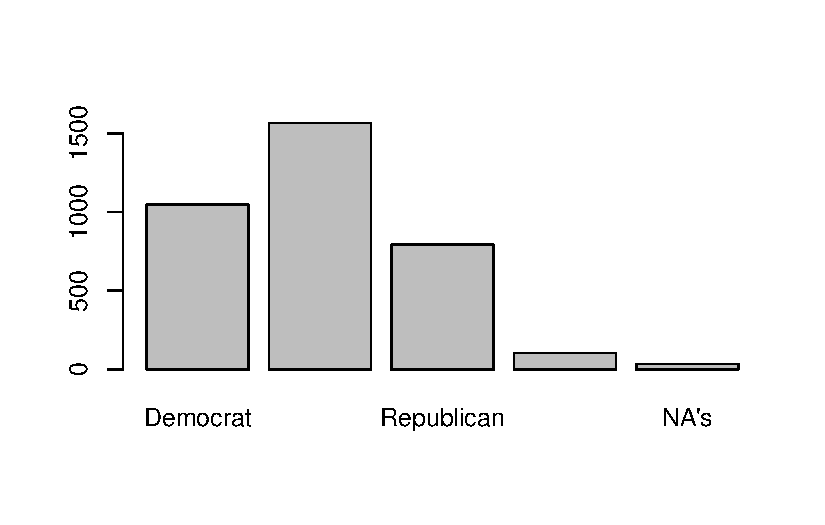
\includegraphics[keepaspectratio]{univariate_categorical_files/figure-pdf/unnamed-chunk-13-1.pdf}}

Now, as I mentioned, we won't spend too much time adjusting these plots
for now, but there are a couple things we can do to make this a little
better to look at for now.

For one, our response labels (Democrat, Republican, Independent, etc)
Actually look pretty good in the display here, but it's not uncommon for
these to get cut off if we have several response categories or the
response names are especially long. So, I'll show you how to reduce the
font size as one potential fix for that.

We can add the \texttt{cex.names} argument to \texttt{barplot()}. This
argument takes a number, and the number should reflect an intended ratio
of the default font size for our value labels on the x-axis. So, for
example, I would enter `2' if I wanted the font to be twice as big. For
our purposes, I want to reduce the font a bit, so we'll enter `.75' to
reduce the font size by 1/4.

\begin{Shaded}
\begin{Highlighting}[]
\NormalTok{our\_gss}\SpecialCharTok{$}\NormalTok{partyid\_recoded }\SpecialCharTok{|\textgreater{}}
  \FunctionTok{summary}\NormalTok{() }\SpecialCharTok{|\textgreater{}}
  \FunctionTok{barplot}\NormalTok{(}\AttributeTok{cex.names =}\NormalTok{ .}\DecValTok{75}\NormalTok{)}
\end{Highlighting}
\end{Shaded}

\pandocbounded{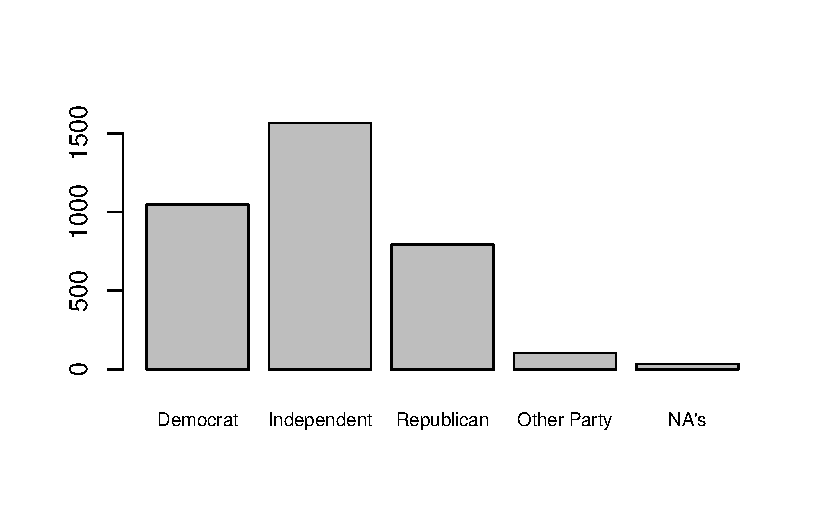
\includegraphics[keepaspectratio]{univariate_categorical_files/figure-pdf/unnamed-chunk-14-1.pdf}}

We can also add some simple descriptive information for the plot, such
as a title and labels for the x and y axis. We can do so within
\texttt{barplot()}

\begin{Shaded}
\begin{Highlighting}[]
\NormalTok{our\_gss}\SpecialCharTok{$}\NormalTok{partyid\_recoded }\SpecialCharTok{|\textgreater{}}
  \FunctionTok{summary}\NormalTok{() }\SpecialCharTok{|\textgreater{}}
  \FunctionTok{barplot}\NormalTok{(}
    \AttributeTok{cex.names =}\NormalTok{ .}\DecValTok{75}\NormalTok{, }
    \AttributeTok{main =} \StringTok{"Count of GSS Respondents by Political Party"}\NormalTok{,}
    \AttributeTok{xlab =} \StringTok{"Political Party"}\NormalTok{,}
    \AttributeTok{ylab =} \StringTok{"Count"}
\NormalTok{  )}
\end{Highlighting}
\end{Shaded}

\pandocbounded{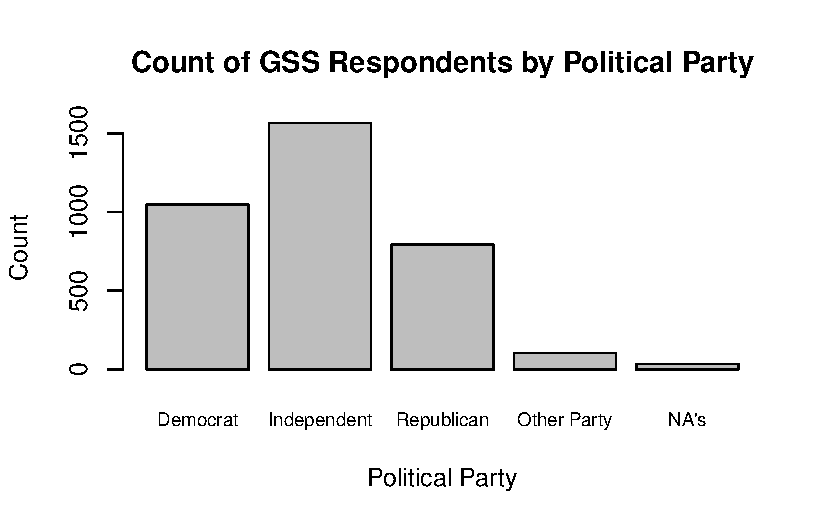
\includegraphics[keepaspectratio]{univariate_categorical_files/figure-pdf/unnamed-chunk-15-1.pdf}}

As a final point, I'll also note that you can pass
\texttt{partyid\_recoded} into the function \texttt{na.omit()} before
\texttt{summary()} if you ever want to produce a barplot that excludes
NA responses. \texttt{na.omit()} will remove any NA values from the
vector we provide it.

\begin{Shaded}
\begin{Highlighting}[]
\NormalTok{our\_gss}\SpecialCharTok{$}\NormalTok{partyid\_recoded }\SpecialCharTok{|\textgreater{}}
  \FunctionTok{na.omit}\NormalTok{() }\SpecialCharTok{|\textgreater{}}
  \FunctionTok{summary}\NormalTok{() }\SpecialCharTok{|\textgreater{}}
  \FunctionTok{barplot}\NormalTok{(}
    \AttributeTok{cex.names =}\NormalTok{ .}\DecValTok{75}\NormalTok{,}
    \AttributeTok{main =} \StringTok{"Count of GSS Respondents by Political Party"}\NormalTok{,}
    \AttributeTok{xlab =} \StringTok{"Political party"}
\NormalTok{  )}
\end{Highlighting}
\end{Shaded}

\pandocbounded{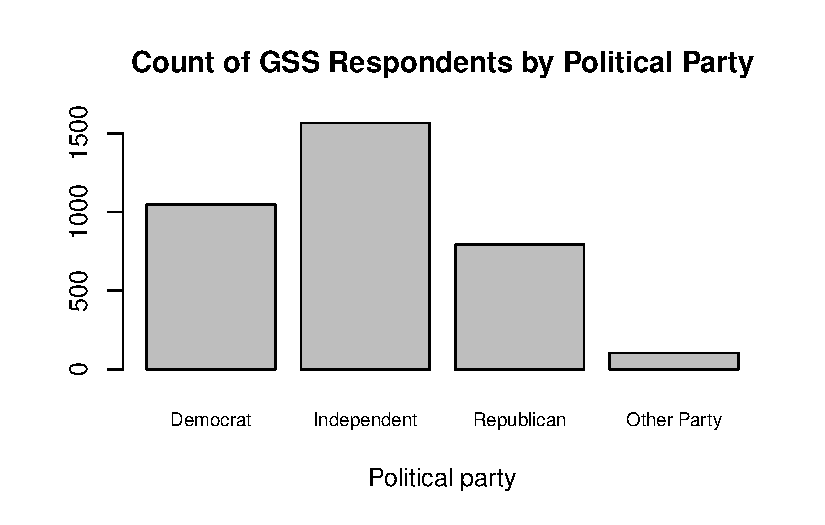
\includegraphics[keepaspectratio]{univariate_categorical_files/figure-pdf/unnamed-chunk-16-1.pdf}}

\section{Measures of Central
Tendency}\label{measures-of-central-tendency}

Now, let's talk about measures of central tendency. Because there is no
mathematically meaningful relationship between the different levels of a
categorical variable, our options for reporting measures of central
tendency are a little more limited.

The classic central tendency measures are the mode, the median, and the
mean. For categorical variables, it is not ever meaningful to take the
mean. As we saw back on our first day with R, you will get a warning
message if you try to run \texttt{mean()} on a character or factor
variable.

Our options are limited to the mode or the median, depending on the
distribution of responses.

\subsection{Nominal variables}\label{nominal-variables}

In the case nominal variables, there is no semblance of meaningful
arrangement to the categories. In this case, we can only report the
mode.

Often times, we can just glean this from the frequency tables, or even
just the \texttt{summary()} output. Let's stick with
\texttt{partyid\_recoded} as an example.

\begin{Shaded}
\begin{Highlighting}[]
\FunctionTok{summary}\NormalTok{(our\_gss}\SpecialCharTok{$}\NormalTok{partyid\_recoded)}
\end{Highlighting}
\end{Shaded}

\begin{verbatim}
   Democrat Independent  Republican Other Party        NA's 
       1046        1565         792         106          35 
\end{verbatim}

Remember that the mode is just the value with the most occurrences. So,
the mode here is `Independent'.

This is likely sufficient for the variables we will work with, but you
may also want a method that's a little more exacting and does not depend
on visually scanning for the mode.

R does not actually have a built-in \texttt{mode()} function like it
does for \texttt{mean()} and \texttt{median()}. Well, it does have
\texttt{mode()}, but it evaluates the `mode' of the data, which, in this
case, is actually the `storage mode', or the data type. This is not
particularly helpful for us, but we can use another convenient package
called \texttt{DescTools}.

If you are on a lab computer, go ahead and try loading it with
\texttt{library()} first. If it does not load, then install it with
\texttt{install.packages("DescTools")} and then load it in.

\begin{Shaded}
\begin{Highlighting}[]
\FunctionTok{library}\NormalTok{(DescTools)}
\end{Highlighting}
\end{Shaded}

Then, we can just use the \texttt{Mode()} function within DescTools.
Make sure you capitalize the `M', as this is what distinguishes the
DescTools function from the base R function.

Also, be sure to include \texttt{na.rm\ =\ TRUE}, as R will not know
what to do with the NA values when calculating the mode, so we need to
tell it to disregard them.

\begin{Shaded}
\begin{Highlighting}[]
\FunctionTok{Mode}\NormalTok{(our\_gss}\SpecialCharTok{$}\NormalTok{partyid\_recoded, }\AttributeTok{na.rm =} \ConstantTok{TRUE}\NormalTok{)}
\end{Highlighting}
\end{Shaded}

\begin{verbatim}
[1] Independent
attr(,"freq")
[1] 1565
Levels: Democrat Independent Republican Other Party
\end{verbatim}

So, this also gives us our mode, and is a bit more precise a way of
doing so---especially when we have a bunch of possible response values.

Note that it also tells us how many responses were associated with that
value (1565).

Now, let's talk about ordinal variables, where we have another
consideration.

\subsection{Ordinal variables}\label{ordinal-variables}

While ordinal variables are still categorical and thus unamenable to
mathematical analysis, they do have a meaningful order. This means that
it's possible for us to take the median value of an ordinal variable.

However, we can only do so when the variable is normally distributed. If
there is significant skew in the distribution of responses, then we will
need to report the mode for an ordinal variable.

Let's refresh our memory on distributions before we take some central
tendency measures of ordinal variables in the GSS.

\paragraph{Distribution assumptions}\label{distribution-assumptions}

If the responses of an ordinal variable are normally distributed, we can
take the median.

In the ideal form of the normal distribution, you have a mean of 0 and a
standard deviation of 1, where roughly 68\% of values are within 1
standard deviation in either direction of the mean, and roughly 95\% of
values are within 2 standard deviations in either direction.

However, in practice, our distributions are unlikely to reflect the
ideal normal distribution. But, if they are roughly normal, we can work
with that.

I'll display a few distributions here as a reminder, starting with the
classic normal distribution. If you produce a barplot and find the data
looks generally like this---where the majority of variables are
concentrated around the middle of the distribution---then you can report
the median response rather than the mode.

Here's the normal distribution

\pandocbounded{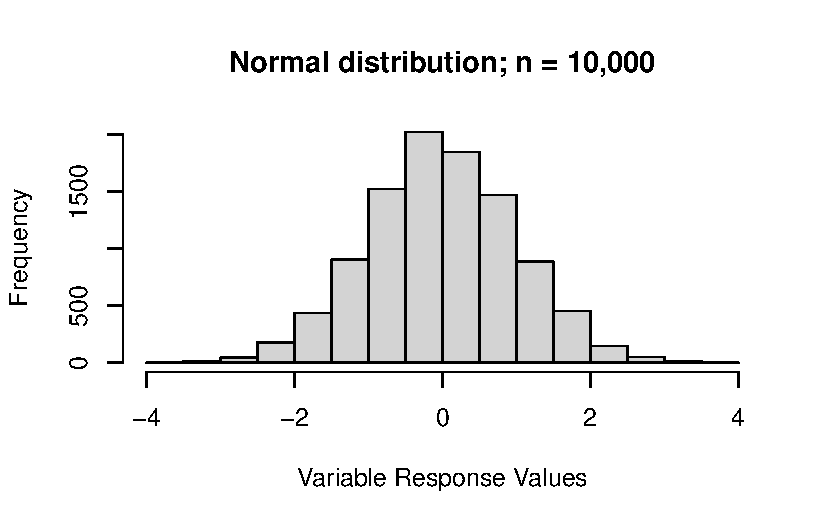
\includegraphics[keepaspectratio]{univariate_categorical_files/figure-pdf/unnamed-chunk-20-1.pdf}}

Here's a left-skewed distribution. This is when there's a prominent
`tail' on most of the left-hand side of the distribution. In other
words, when most of the values are concentrated on the right-hand side
of the distribution (the upper end), then we have a left-skew.

\pandocbounded{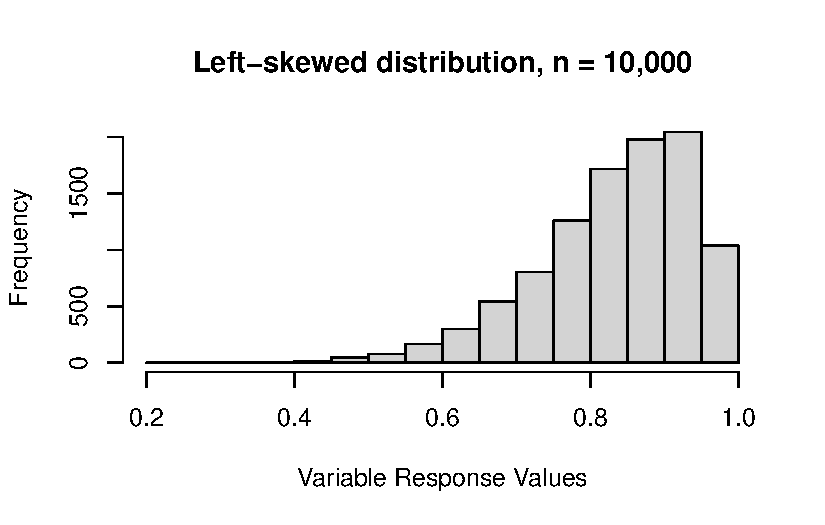
\includegraphics[keepaspectratio]{univariate_categorical_files/figure-pdf/unnamed-chunk-21-1.pdf}}

Lastly, here's a right-skewed distribution. As you can probably guess
from the description of a left-skewed distribution, a right-skew occurs
when we have a long tail through most of the right-hand side of the
distribution. In other words, most values are concentrated on the
left-hand side.

\pandocbounded{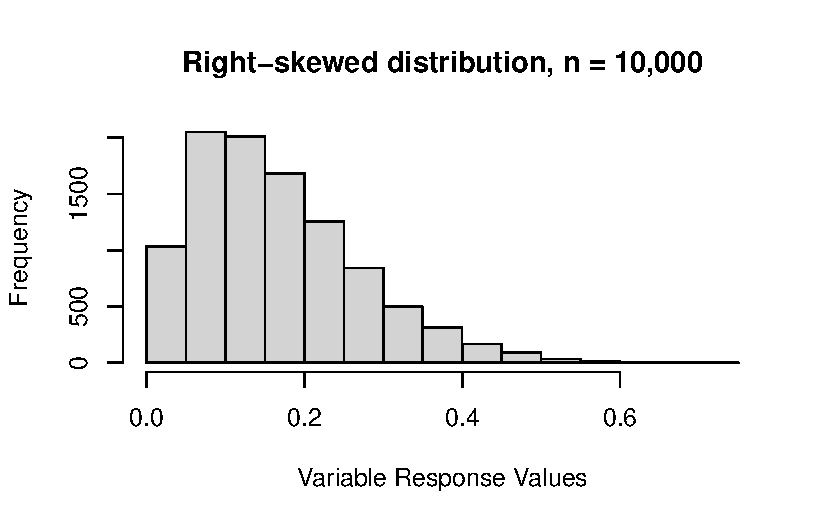
\includegraphics[keepaspectratio]{univariate_categorical_files/figure-pdf/unnamed-chunk-22-1.pdf}}

So, if the distribution of your variable looks (mostly) like the normal
distribution, go ahead and take the median of any ordinal variable.

Let's go ahead and practice doing that with the \texttt{age\_ord}
variable we created last time.

First, we'll verify that the distribution allows for reporting the
median.

\begin{Shaded}
\begin{Highlighting}[]
\NormalTok{our\_gss}\SpecialCharTok{$}\NormalTok{age\_ord }\SpecialCharTok{|\textgreater{}}
  \FunctionTok{na.omit}\NormalTok{() }\SpecialCharTok{|\textgreater{}}
  \FunctionTok{summary}\NormalTok{() }\SpecialCharTok{|\textgreater{}}
  \FunctionTok{barplot}\NormalTok{(}
    \AttributeTok{main =} \StringTok{"Age Distribution of GSS Respondents"}\NormalTok{,}
    \AttributeTok{xlab =} \StringTok{"Age grouping"}
\NormalTok{  )}
\end{Highlighting}
\end{Shaded}

\pandocbounded{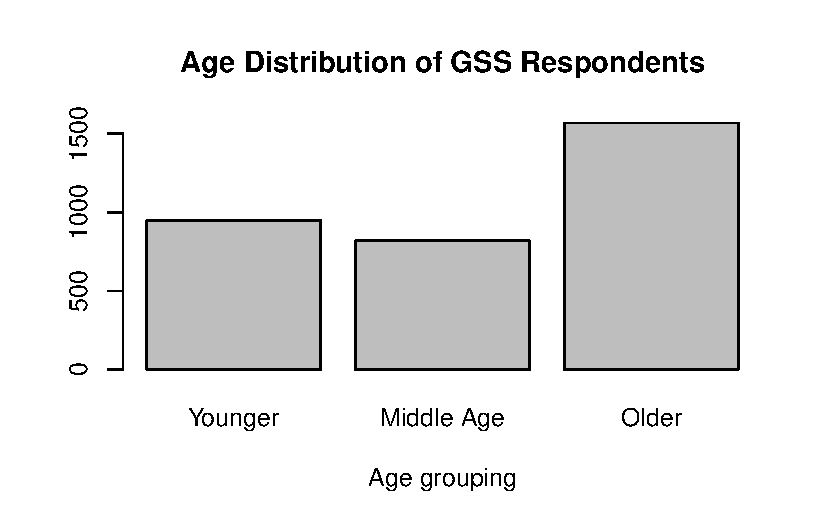
\includegraphics[keepaspectratio]{univariate_categorical_files/figure-pdf/unnamed-chunk-24-1.pdf}}

Well, hold on now. In the case of \texttt{age\_ord}, it looks like we'd
actually want to take the mode, because it's a bit left-skewed.

Let's try the \texttt{happy} variable. This is an ordinal variable in
our subset that we haven't used yet. We'll see if its normally
distributed.

\begin{Shaded}
\begin{Highlighting}[]
\NormalTok{ our\_gss}\SpecialCharTok{$}\NormalTok{happy }\SpecialCharTok{|\textgreater{}}
  \FunctionTok{na.omit}\NormalTok{() }\SpecialCharTok{|\textgreater{}}
  \FunctionTok{summary}\NormalTok{() }\SpecialCharTok{|\textgreater{}}
  \FunctionTok{barplot}\NormalTok{(}
    \AttributeTok{main =} \StringTok{"Happiness Distribution of 2022 GSS Respondents"}\NormalTok{,}
    \AttributeTok{xlab =} \StringTok{"Response value"}
\NormalTok{  )}
\end{Highlighting}
\end{Shaded}

\pandocbounded{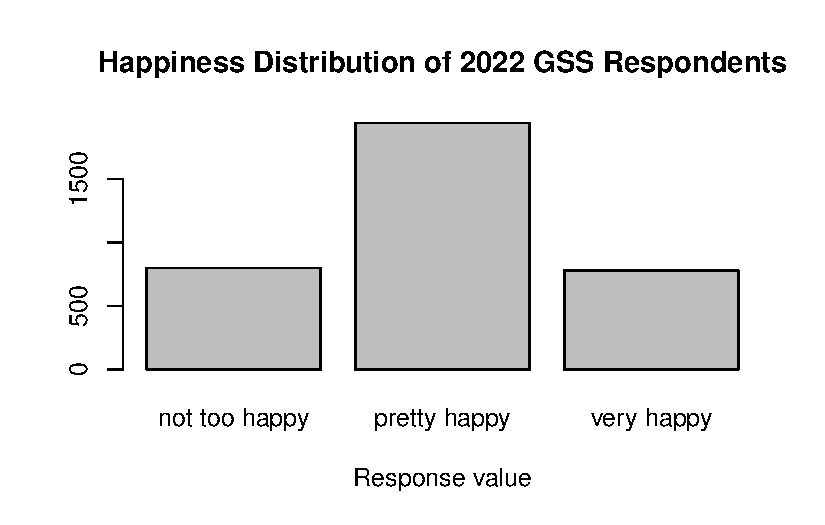
\includegraphics[keepaspectratio]{univariate_categorical_files/figure-pdf/unnamed-chunk-25-1.pdf}}

Perfect. The distribution is exactly what we want to see. Most of the
variables are concentrated at the midpoint of the distribution, with
tails on either side. So, as it's roughly normally distributed,
\texttt{happy} will serve as a good example of a case where taking the
median of an ordinal variable is appropriate.

Now, the median response value is fairly apparent in this case, but I'll
show you a method that you can use to calculate the median of any
ordinal variable you might come across.

While R has a built-in \texttt{median()} function, it actually only
works with numeric data. Fear not, however, as we can also use the
\texttt{DescTools} again.

In order to distinguish itself from the default \texttt{median()}
function, the DescTools package uses a capitalized `M'. So, make sure
you use \texttt{Median()} when you are working with an ordinal variable.

We also need to assure that NAs are not included for the calculation. As
we have seen a few times, R will not know what to do with these if we
don't tell it to exclude them.

\begin{Shaded}
\begin{Highlighting}[]
\FunctionTok{Median}\NormalTok{(our\_gss}\SpecialCharTok{$}\NormalTok{happy, }\AttributeTok{na.rm =} \ConstantTok{TRUE}\NormalTok{)}
\end{Highlighting}
\end{Shaded}

\begin{verbatim}
[1] pretty happy
Levels: not too happy < pretty happy < very happy
\end{verbatim}

Perfect! Looks like our median is `pretty happy'.

And now we have all we need to report a univariate analysis of a
categorical variable in this course:

\begin{itemize}
\tightlist
\item
  A frequency table
\item
  A bar plot
\item
  A median or mode
\end{itemize}

For now, it's just important that you can accurately identify the median
or mode of a categorical value. We'll talk about ways to implement it in
the tables a little later on when we focus on publication-ready tables
and figures.

Now, let's talk about presenting a univariate analysis of numeric data.

\chapter{Univariate: Numeric}\label{univariate-numeric}

While we also want to report on the frequency distribution and central
tendency of numeric variables, there are some differences in the way we
go about that relative to the techniques we just learned about for
categorical variables.

Additionally, we will need to report on some measures of dispersion that
can only be reported for numeric data, such as the standard deviation.

This section will walk us through the process of calculating and
reporting necessary elements of a univariate analysis of numeric data.

\section{Frequency Distributions}\label{frequency-distributions-1}

As we saw when we were recoding \texttt{age} earlier in the unit, a
frequency table is not really appropriate for numeric data. When there
are upwards of 71 different response values---as we have with
\texttt{age}---a table would be both spatially unwieldy and difficult to
interpret.

So, let's start with a style of plotting data that is essentially the
barplot of numeric data.

First, let's go ahead and set up our environment by loading in our data
and \texttt{tidyverse} per usual.

\begin{Shaded}
\begin{Highlighting}[]
\FunctionTok{library}\NormalTok{(tidyverse)}
\FunctionTok{load}\NormalTok{(}\StringTok{"our\_gss.rda"}\NormalTok{)}
\end{Highlighting}
\end{Shaded}

\subsection{Histograms}\label{histograms}

A histogram is the result of taking a numeric variable, slicing it up
into equal, ordinal intervals, and then plotting the frequency of each
interval.

There are plenty of other ways for plotting numeric data---some of which
we will see later when we focus on visualization---but for now, this is
a simple and effective way to get a sense of the distribution of a
numeric variable. This is especially important when we need to decide on
an appropriate measure of central tendency.

We can create these easily using the \texttt{hist()} function, which is
in the same family of base R plotting functions as \texttt{barplot()},
so much of what we learned for that function will also apply with
\texttt{hist()}. This function will automatically apply a commonly used
method called Sturges's rule to divide our numeric variable into equal
bins, so we do not have to specify anything in that regard.

All we need to do is give the \texttt{hist()} function our numeric
variable. Let's work with the \texttt{realrinc} variable for this
example.

\begin{Shaded}
\begin{Highlighting}[]
\FunctionTok{hist}\NormalTok{(our\_gss}\SpecialCharTok{$}\NormalTok{realrinc)}
\end{Highlighting}
\end{Shaded}

\pandocbounded{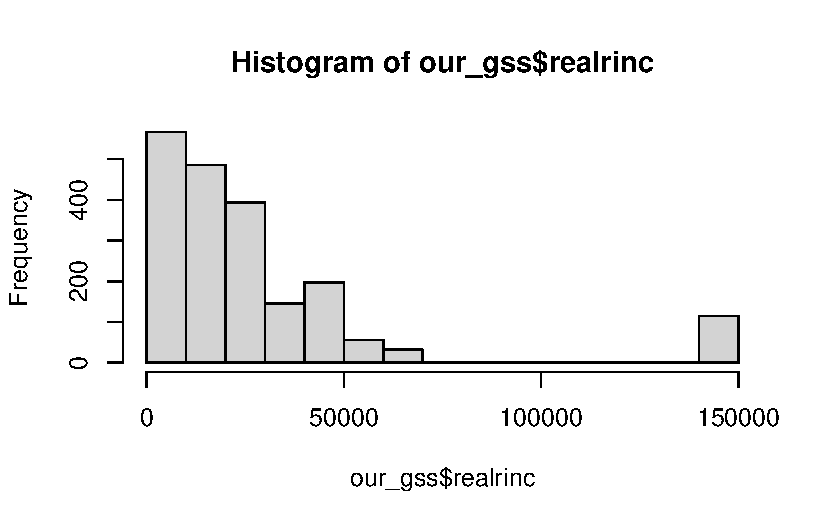
\includegraphics[keepaspectratio]{univariate_numeric_files/figure-pdf/unnamed-chunk-2-1.pdf}}

Much like we did with \texttt{barplot()}, we can clean this up a little
by adding a title and a better label for the x axis

\begin{Shaded}
\begin{Highlighting}[]
\FunctionTok{hist}\NormalTok{(}
\NormalTok{  our\_gss}\SpecialCharTok{$}\NormalTok{realrinc,}
  \AttributeTok{main =} \StringTok{"Income distribution of GSS Respondents"}\NormalTok{,}
  \AttributeTok{xlab =} \StringTok{"Respondent\textquotesingle{}s income in dollars"}\NormalTok{,}
\NormalTok{  )}
\end{Highlighting}
\end{Shaded}

\pandocbounded{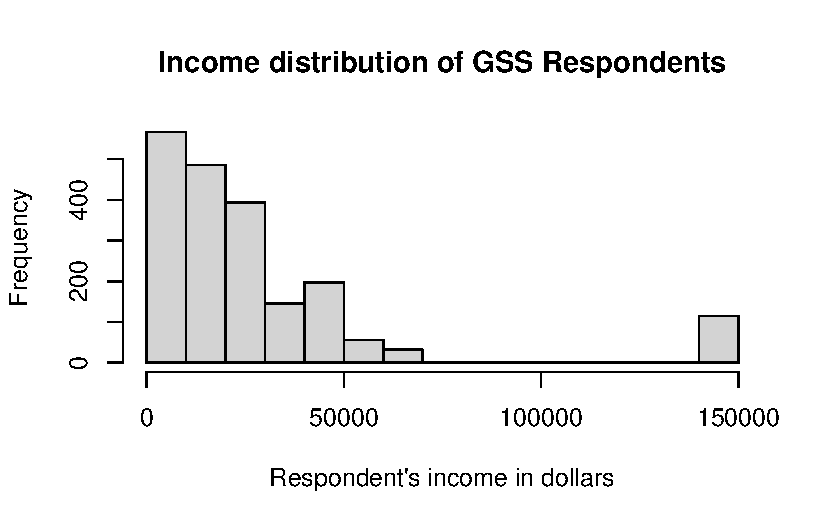
\includegraphics[keepaspectratio]{univariate_numeric_files/figure-pdf/unnamed-chunk-3-1.pdf}}

Now we have our histogram!

However, this visualization does suggest that we need to do some
thinking about the appropriate measure of central tendency for
\texttt{realrinc}.

\section{Central Tendency}\label{central-tendency}

For numeric data, any of the 3 common measures of central tendency can
be reported. However, the preferred measure for a given variable depends
on its distribution.

The mean is the gold standard for numeric data, because it takes into
account every single data point in its calculation, and is thus the most
comprehensive index of central tendency.

However, the mean can be misleading in some cases. The distribution
should be (basically) normal in order for you to report the mean, and
you will want to report the median in most other cases.

I will first cover the choice of mean or median by revisiting some
basics of distributions, and then I will address the rare circumstance
where the mode is appropriate.

\subsection{Mean or Median?}\label{mean-or-median}

In most cases, we will be making a decision between the mean and the
median. When the distribution is normal, you should report the
mean---otherwise, report the median. We'll see one exception to this
later, but that's generally our task.

We saw some typical distributions in our last section on uivariate
analysis of categorical data. We'll return to some discussion of those
basic distribution types but add a little more context for numeric data
that will help us see the impact of making the wrong decision.

I'm going to display a normal distribution, but this time, I'll draw a
vertical line indicating the location of the mean and median.

\pandocbounded{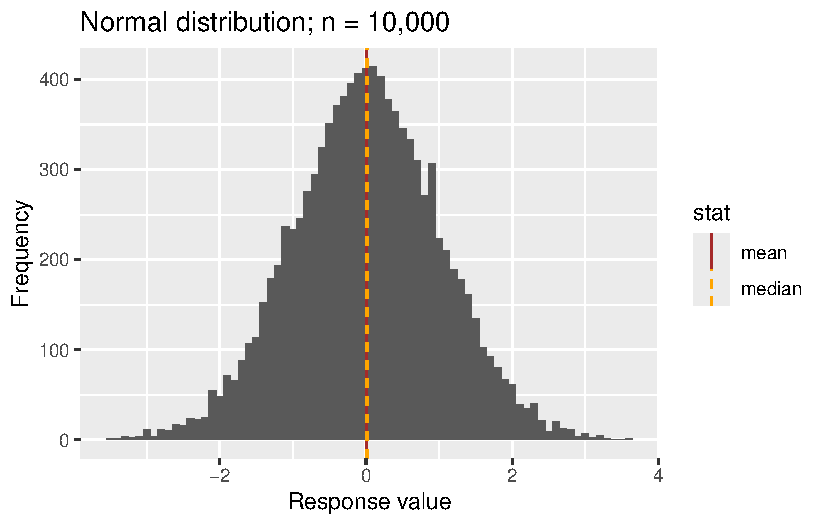
\includegraphics[keepaspectratio]{univariate_numeric_files/figure-pdf/unnamed-chunk-4-1.pdf}}

In this case, we can't even really tell the mean and median apart. In
fact, in a completely normal distribution, all three measures of central
tendency will be equal. Remember that real-world data will rarely
exhibit perfect normality, but as long as it's approximately normal, we
can follow convention and report the mean.

Now, let's look back at \texttt{realrinc}.

\pandocbounded{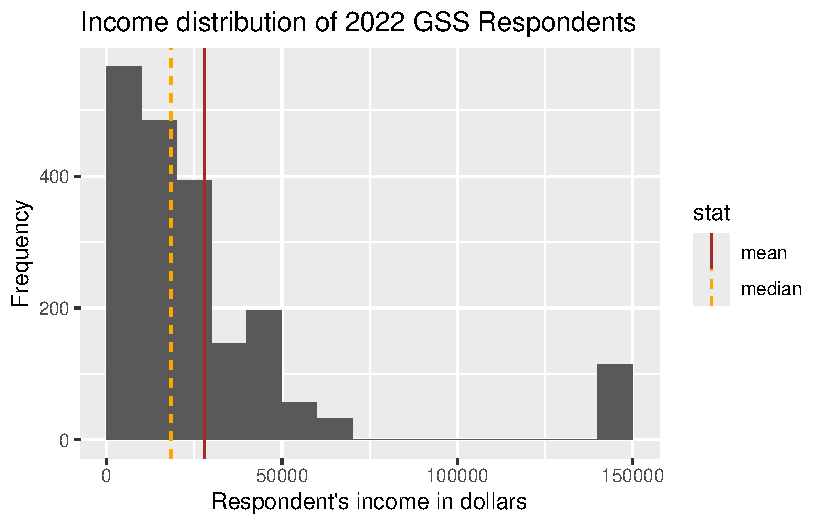
\includegraphics[keepaspectratio]{univariate_numeric_files/figure-pdf/unnamed-chunk-5-1.pdf}}

In the case of \texttt{realrinc}, we definitely do not have much
normality going on. For one, there are some apparent outlier cases. Much
of our data seems to be concentrated within about \$0 - \$75,000, but
then we have a bunch of values at roughly double the maximum of that
narrower range. And even within the range where most of our responses
are clustered, we have some clear right-skew.

As we can see, because the mean takes all values into account, this
makes it susceptible to non-normal distributions. It gets pulled in the
direction of the outlier, which, in this case, is also the direction of
the skew.

So, in any case where your numeric variable contains clear outliers
and/or exhibits notable skew in either direction, you should report the
median rather than the mean.

\subsection{The Mode}\label{the-mode}

By and large, the mode is more appropriate for categorical data. But
there are some circumstances where it makes sense to report the mode for
numeric data.

Let's take a look at the original \texttt{age} variable to see an
example.

\begin{Shaded}
\begin{Highlighting}[]
\FunctionTok{hist}\NormalTok{(}
\NormalTok{  our\_gss}\SpecialCharTok{$}\NormalTok{age,}
  \AttributeTok{main =} \StringTok{"Age distribution of 2022 GSS Respondents"}\NormalTok{,}
  \AttributeTok{xlab =} \StringTok{"Respondent age in years"}
\NormalTok{)}
\end{Highlighting}
\end{Shaded}

\pandocbounded{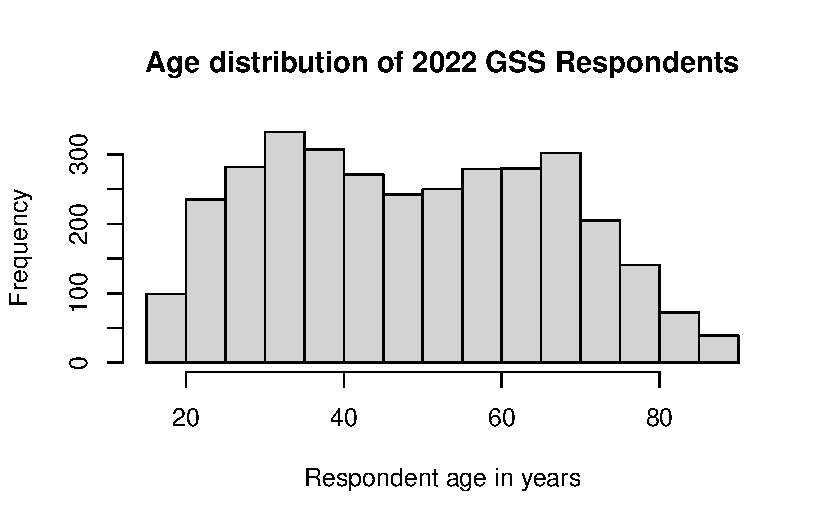
\includegraphics[keepaspectratio]{univariate_numeric_files/figure-pdf/unnamed-chunk-6-1.pdf}}

This isn't quite a normal distribution, but it's not exactly skewed in
either direction either. And there are no apparent outliers.

What we have here is a \textbf{bimodal} distribution.

This is what happens when we have multiple peaks in a
distribution---two, in this case. We have seen several different
distributions so far, but they all had only one peak in the
distribution. They were differentiated on the basis of that single
peak's location in the distribution. In the case of a multimodal
distribution, we want to report on any notable peak.

This may be a peculiarity of the 2022 survey wave, because we wouldn't
necessarily expect this, but it looks like there are two distinct
central tendencies for \texttt{age}. In this case, we want to capture
the two distinct peaks, meaning we need to calculate two modes.

Thankfully, there's a convenient function for this, but we need to
install a new package, so let's install and load in \texttt{multimode}.

\begin{Shaded}
\begin{Highlighting}[]
\FunctionTok{install.packages}\NormalTok{(}\StringTok{"multimode"}\NormalTok{)}
\FunctionTok{library}\NormalTok{(multimode)}
\end{Highlighting}
\end{Shaded}

Then, we just need to provide a few arguments to the \texttt{locmodes()}
function.

First, we give the variable for which we want to calculate multiple
modes.

Then we give an input for \texttt{mod0}, which asks us how many modes
the function should be looking for. This should be based on visual
inspection of the data. We have two peaks in our distribution, so we
will enter `2' for this input.

Lastly, we will set \texttt{display} to `TRUE', which will show us a
plot of the estimated modes superimposed onto the frequency distribution
of the variable. This will let us evaluate whether the modes estimated
by the function are plausible. They should match up with the visible
peaks in the frequency distribution.

\begin{Shaded}
\begin{Highlighting}[]
\FunctionTok{locmodes}\NormalTok{(}
\NormalTok{  our\_gss}\SpecialCharTok{$}\NormalTok{age,}
  \AttributeTok{mod0 =} \DecValTok{2}\NormalTok{,}
  \AttributeTok{display =} \ConstantTok{TRUE}
\NormalTok{)}
\end{Highlighting}
\end{Shaded}

\pandocbounded{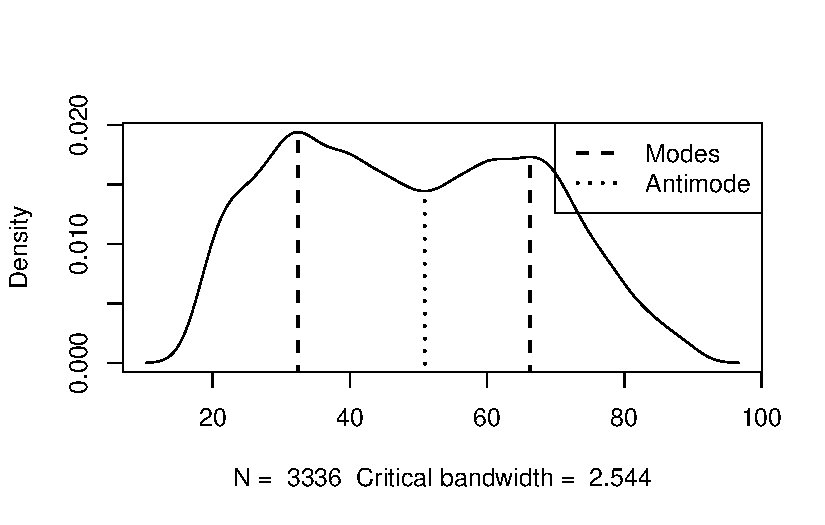
\includegraphics[keepaspectratio]{univariate_numeric_files/figure-pdf/unnamed-chunk-9-1.pdf}}

\begin{verbatim}

Estimated location
Modes:  32.4301  66.25356 
Antimode: 50.89506 

Estimated value of the density
Modes: 0.01938966  0.01730832 
Antimode: 0.01444287 

Critical bandwidth: 2.543659
\end{verbatim}

We only really need to pay attention to the modes that it gives us
(32.43 and 66.25), but it looks like this function spotted these values
pretty effectively.

For a bimodal distribution like this, we can report both modes for the
measure of central tendency. I don't expect we will run into too much of
this, but go ahead and deal with it like this in the event that you do.

\section{Dispersion}\label{dispersion}

Now, let's talk about dispersion. This is the last major element of a
univariate analysis of numeric data. Actually calculating this
information is quite simple in R, so we will practice with some of our
GSS variables and then talk about putting all of this information
together.

\subsection{Range}\label{range}

This is perhaps the simplest measure of dispersion and comprises the
minimum and maximum values of the distribution.

R has a built in range function, so we can simply provide one of our
variables as the input. We'll work with \texttt{realrinc} again. As we
have done before, we will also need to provide \texttt{na.rm\ =\ TRUE},
as this variable column includes NAs and will confuse R otherwise.

\begin{Shaded}
\begin{Highlighting}[]
\FunctionTok{range}\NormalTok{(our\_gss}\SpecialCharTok{$}\NormalTok{realrinc, }\AttributeTok{na.rm =} \ConstantTok{TRUE}\NormalTok{)}
\end{Highlighting}
\end{Shaded}

\begin{verbatim}
[1]    204.5 141848.3
\end{verbatim}

At this point, I'll also offer a reminder about the \texttt{summary()}
function, which we can use to see a variety of information about the
dispersion (in an addition to the central tendency).

\begin{Shaded}
\begin{Highlighting}[]
\FunctionTok{summary}\NormalTok{(our\_gss}\SpecialCharTok{$}\NormalTok{realrinc)}
\end{Highlighting}
\end{Shaded}

\begin{verbatim}
    Min.  1st Qu.   Median     Mean  3rd Qu.     Max.     NA's 
   204.5   8691.2  18405.0  27835.3  33742.5 141848.3     1554 
\end{verbatim}

For a numeric variable, \texttt{summary()} will show us the minimum \&
maximum, as well as the mean \& median, and the 1st \& 3rd quartiles.

We can actually think of most of these elements in terms of percentiles.

\begin{itemize}
\item
  The minimum value is the 0th percentile of the distribution
\item
  The 1st quartile is the 25th percentile.
\item
  The median is the 50th percentile
\item
  The 3rd quartile is the 75th percentile
\item
  And the maximum is the 100th percentile.
\end{itemize}

\texttt{summary()} is great for quickly assessing some of these
descriptive statistics, but it's a little less convenient for exporting
this information into something like a table for our own univariate
analysis.

So, I'll also highlight the \texttt{min()} and \texttt{max()} functions,
which will come in hand for us shortly. They work simply enough---we
just need to provide our variable column, and they will output the
minimum and maximum, respectively.

\begin{Shaded}
\begin{Highlighting}[]
\FunctionTok{min}\NormalTok{(our\_gss}\SpecialCharTok{$}\NormalTok{realrinc, }\AttributeTok{na.rm =} \ConstantTok{TRUE}\NormalTok{)}
\end{Highlighting}
\end{Shaded}

\begin{verbatim}
[1] 204.5
\end{verbatim}

\begin{Shaded}
\begin{Highlighting}[]
\FunctionTok{max}\NormalTok{(our\_gss}\SpecialCharTok{$}\NormalTok{realrinc, }\AttributeTok{na.rm =} \ConstantTok{TRUE}\NormalTok{)}
\end{Highlighting}
\end{Shaded}

\begin{verbatim}
[1] 141848.3
\end{verbatim}

\subsection{Standard Deviation}\label{standard-deviation}

This is one of the more commonly reported dispersion metrics for numeric
data. The standard deviation is a measure of how much the average value
varies from the mean. In plainer terms, it's a measure that tells us how
spread out the distribution is.

\pandocbounded{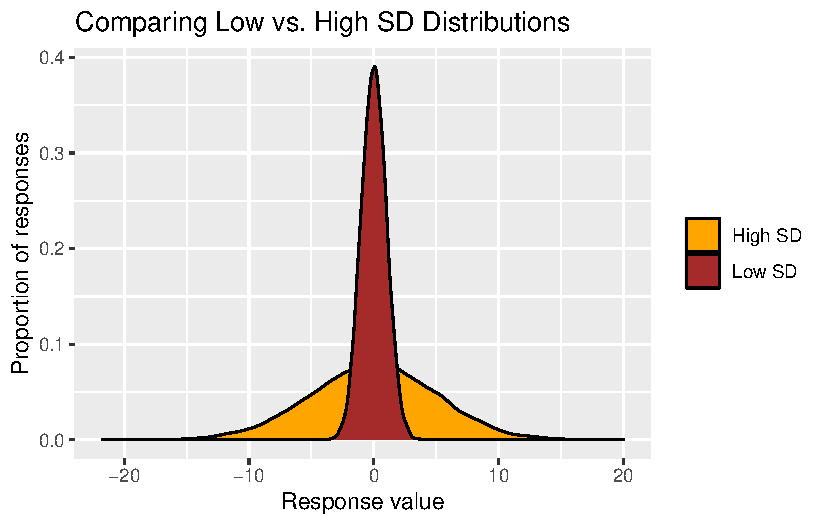
\includegraphics[keepaspectratio]{univariate_numeric_files/figure-pdf/unnamed-chunk-13-1.pdf}}

We can grab the standard deviation quite easily with the \texttt{sd()}
function

\begin{Shaded}
\begin{Highlighting}[]
\FunctionTok{sd}\NormalTok{(our\_gss}\SpecialCharTok{$}\NormalTok{realrinc, }\AttributeTok{na.rm =} \ConstantTok{TRUE}\NormalTok{)}
\end{Highlighting}
\end{Shaded}

\begin{verbatim}
[1] 31962.34
\end{verbatim}

Now, let's talk about putting all this together in our reporting of a
univariate analysis for numeric data.

\section{Putting It All Together}\label{putting-it-all-together-1}

Now that we have worked through how to calculate all of these key
statistics with R, let's revisit some of the first \texttt{tidyverse}
functions we learned about back on the first day.

We can use a combination of \texttt{select()} and \texttt{summarize} to
quickly compile several bits of important information, such as the
range, the central tendency, and the standard deviation.

Let's do this for \texttt{realrinc}.

\begin{Shaded}
\begin{Highlighting}[]
\NormalTok{our\_gss }\SpecialCharTok{|\textgreater{}}
  \FunctionTok{select}\NormalTok{(realrinc) }\SpecialCharTok{|\textgreater{}}
  \FunctionTok{summarize}\NormalTok{(}
    \StringTok{"Minimum"} \OtherTok{=} \FunctionTok{min}\NormalTok{(realrinc, }\AttributeTok{na.rm =} \ConstantTok{TRUE}\NormalTok{),}
    \StringTok{"Median"} \OtherTok{=} \FunctionTok{median}\NormalTok{(realrinc, }\AttributeTok{na.rm =} \ConstantTok{TRUE}\NormalTok{),}
    \StringTok{"Maximum"} \OtherTok{=} \FunctionTok{max}\NormalTok{(realrinc, }\AttributeTok{na.rm =} \ConstantTok{TRUE}\NormalTok{),}
    \StringTok{"SD"} \OtherTok{=} \FunctionTok{sd}\NormalTok{(realrinc, }\AttributeTok{na.rm =} \ConstantTok{TRUE}\NormalTok{)}
\NormalTok{  )}
\end{Highlighting}
\end{Shaded}

\begin{verbatim}
  Minimum Median  Maximum       SD
1   204.5  18405 141848.3 31962.34
\end{verbatim}

\begin{tcolorbox}[enhanced jigsaw, colframe=quarto-callout-note-color-frame, arc=.35mm, coltitle=black, breakable, rightrule=.15mm, left=2mm, opacitybacktitle=0.6, colbacktitle=quarto-callout-note-color!10!white, toptitle=1mm, bottomtitle=1mm, titlerule=0mm, leftrule=.75mm, colback=white, title=\textcolor{quarto-callout-note-color}{\faInfo}\hspace{0.5em}{Note}, opacityback=0, bottomrule=.15mm, toprule=.15mm]

You might notice that there's an attribute for each column that looks
like \texttt{\textless{}dbl\textgreater{}}. This is short for `double',
which is itself shorthand for `double-precision floating-point format'.
This is in reference to the underlying data type that R uses to store
continuous numeric values. You really don't need to know anything more
about double-precision floating point than that for our purposes, but I
mention it here because you might run into or `double' in R. When you
do, just think `numeric data'.

\end{tcolorbox}

If you have a numeric variable where the mean is more appropriate, you
can just swap \texttt{median()} with \texttt{mean()} in the code
template above. Be sure to also change the column name as well.

And that should do us! For any univariate analysis you report in this
course, you will just need to produce

\begin{itemize}
\tightlist
\item
  a histogram displaying the variable's frequency distribution
\item
  a table like the one above (With the appropriate measure of central
  tendency).
\end{itemize}

\part{Day 3: Bivariate Analysis with the GSS}

\part{Day 4: Multivariable Analysis and Elaboration}

\part{Day 5: Making Better Visualizations}

\chapter*{Introduction}\label{introduction}
\addcontentsline{toc}{chapter}{Introduction}

\markboth{Introduction}{Introduction}

Up to this point, we have worked with pretty simple visualizations, just
so we can quickly glean important information about our statistical
models without spending too much time focusing on the aesthetics of the
visuals.

In this lab, we will learn a bit more about R's graphical
capability---especially through tidyverse's \texttt{ggplot}---which
provides us with incredible customizability. We will learn how to
fine-tune some of the visuals we have already worked with, and we will
preview some other common visual styles that can manage with
\texttt{ggplot}.

\section*{Visualization and Analytical
Thinking}\label{visualization-and-analytical-thinking}
\addcontentsline{toc}{section}{Visualization and Analytical Thinking}

\markright{Visualization and Analytical Thinking}

Before we start working with some of these new visual tools, I want to
take an opportunity to stress the importance of visualization more
generally. It's easy to see the process of presenting visuals as
something somewhat superficial, but visualization can be critical for
defining the kind of questions we can ask about our data.

For now, I'm going to obscure the code I'm using for this document. We
will learn more about the kind of commands I used to generate the
following figures, but I don't want anyone to get bogged down initially.
I'll use these visuals to help impart an important lesson about data
visualization's in the research process.

\section*{Thirteen Data Sets}\label{thirteen-data-sets}
\addcontentsline{toc}{section}{Thirteen Data Sets}

\markright{Thirteen Data Sets}

Let's take a look at a collection of thirteen different data sets. Each
data set has 142 observations with 2 columns, labeled x \& y.

I'll use some tidyverse commands to get some summary statistics for each
of the data sets, including the mean of both variables and their
standard deviations. Let's see what seems to distinguish some of these
data sets from one another.

\begin{verbatim}
# A tibble: 13 x 4
   mean_x mean_y std_x std_y
    <dbl>  <dbl> <dbl> <dbl>
 1   54.3   47.8  16.8  26.9
 2   54.3   47.8  16.8  26.9
 3   54.3   47.8  16.8  26.9
 4   54.3   47.8  16.8  26.9
 5   54.3   47.8  16.8  26.9
 6   54.3   47.8  16.8  26.9
 7   54.3   47.8  16.8  26.9
 8   54.3   47.8  16.8  26.9
 9   54.3   47.8  16.8  26.9
10   54.3   47.8  16.8  26.9
11   54.3   47.8  16.8  26.9
12   54.3   47.8  16.8  26.9
13   54.3   47.8  16.8  26.9
\end{verbatim}

Well, there's not much we can say here. All the summary statistics are
identical. Why don't we try modeling a linear relationship between the x
and y variables. Maybe looking at the correlations will tell us
something. I'll display the linear regression lines for each data set
below.

\pandocbounded{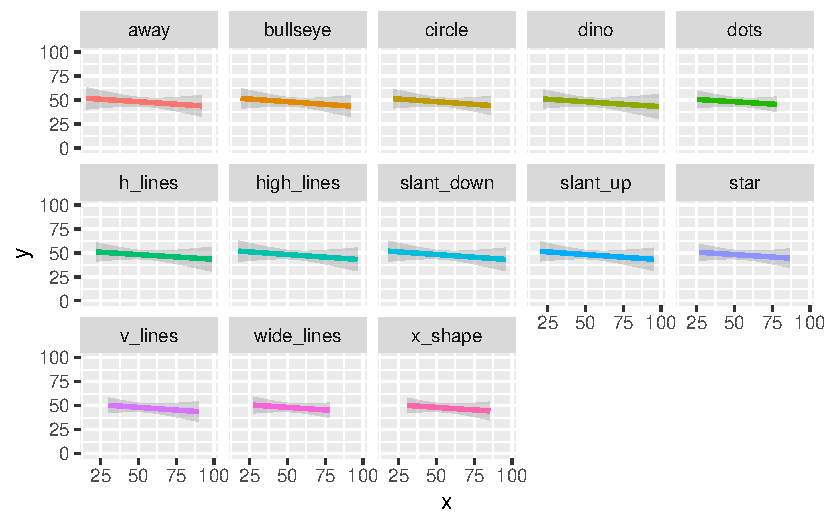
\includegraphics[keepaspectratio]{viz_introduction_files/figure-pdf/unnamed-chunk-2-1.pdf}}

Okay. This is not revealing much either. All the lines seem to have the
same slope, which shows a (slight) negative relationship where y
decreases as x increases. The correlations aren't revealing any notable
distinctions.

But wait. One thing we can see here is that, while the correlations
appear to be about the same, there are some differences in the ranges of
values. Note that the regression lines don't extend across the same
range of x-axis values in each data set. Maybe there is something here
after all.

Let's just go ahead and plot the actual data over our regression lines.

\pandocbounded{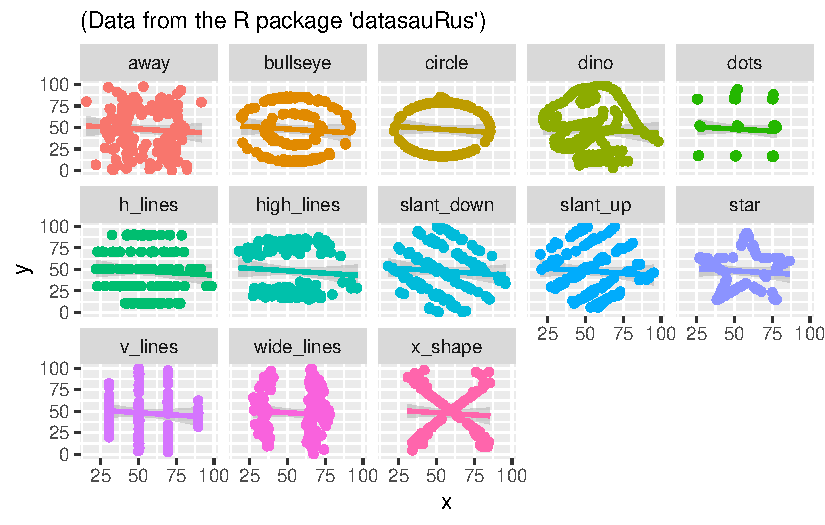
\includegraphics[keepaspectratio]{viz_introduction_files/figure-pdf/unnamed-chunk-3-1.pdf}}

Now there's some distinction!

This is a tongue in cheek data set known as the
\href{https://jumpingrivers.github.io/datasauRus/}{`datasaurus dozen'}.
It's often used in intro statistical classes to help illustrate the
importance of visualization. It's inspired by another conceptually
similar data set known as
\href{https://en.wikipedia.org/wiki/Anscombe\%27s_quartet}{`Anscombe's
quartet'} which likewise stresses the role of plotting data in producing
well informed analyses.

\section*{In Sum}\label{in-sum}
\addcontentsline{toc}{section}{In Sum}

\markright{In Sum}

So, take this as a showcase of the importance of visualizing your data.
This isn't to discount summary statistics and other numeric description
of data---those are still invaluable for us.

Rather, cases like Datasaurus or Anscombe's quartet highlight the
necessity of understanding the shape of your data. This will determine
the kind of questions you can ask with the data, as well as the kind of
statistical tools you need to describe it.

For example, in the case we just examined, those x and y variables do
not have any kind of clear linear relationship. In that case, tools like
regression that assume linearity are not appropriate. Any relationship
between the variables could only be explored through other statistical
means.

So, making our figures and tables look aesthetically pleasing is indeed
valuable in its own right, but don't underestimate the utility of good
visualization for the analytic process itself.




\end{document}
